

\chapter{Pekeris开波导逆散射问题}

从本章开始,我们将研究Pekeris 开波导逆散射问题。在地质勘探、海洋成像以及光纤通信等领域,开波导模型具有非常重要的实际应用。
由于波导模式的存在,当障碍物嵌入在开波导模型当中时,如何确定其位置、大小和形状将变得极其复杂。

通过对点扩散函数的分析和数值测试,我们提出了求解开波导障碍物成像问题的单频逆时偏移算法。该算法能够对不同类型的障碍物进行有效成像,确定其位置、大小和形状,并且不需要提前知道障碍物的先验信息。特别地,当障碍物位于波导第一层时,成像效果类似于闭波导情形
\cite{ch_cw},障碍物的上下边界都能够有效成像;当障碍物位于波导第二层时,成像效果类似于一般半空间情形\cite{ch_ha},对于不可穿透障碍物仅能确定其上半边界。大量的数值算例验证了开波导逆时偏移算法对障碍物成像问题的有效性。

\section{问题介绍}
\begin{figure}[b]
  \centering
  % Requires \usepackage{graphicx}
  \caption{Pekeris模型}
  \includegraphics[width=14cm,height=5cm]{./pekeris/wg_forward}
\label{pekeris_model}
\end{figure}
如图\ref{pekeris_model} 所示,假设可穿透障碍物$D$嵌入在Pekeris模型当中,其中背景介质波数$k(x)$ 为
\begin{eqnarray}
k(x)=\left\{
\begin{array}{lll}
  k_1&,&x_2\in(0,h)\\
  k_2&,&x_2\in(h,+\infty)
\end{array}
\right.
\end{eqnarray}
其中$k_1>k_2$,并记$\Gamma_0,\Gamma_h,L_1,L_2$ 分别为

\begin{itemize}
  \item $ \Gamma_0=\{(x_1,x_2);x_1\in \R, x_2=0\}$;\quad\quad$ \Gamma_h=\{(x_1,x_2);x_1\in \R, x_2=h\}$
  \item $ L_1=\{(x_1,x_2);x_1\in \R, 0<x_2<h\}$;\quad\quad$ L_2=\{(x_1,x_2);x_1\in \R, x_2>h\}$
\end{itemize}


假设可穿透障碍物$D$是一个有界的Lipschitz区域。设源点$x_s\in\Gamma_0$,并记$u(x,x_s)$ 为由源点$x_s$ 激发产生的总场,其满足如下方程
\begin{eqnarray}\label{wg_totalfield}
\left\{
\begin{array}{lll}
 \Delta_x u(x,x_s)+k^2(x)n(x)u(x,x_s)=-\delta_{x_s}(x), &in& \R^2_+,\\
 & &\\
 \left[u(\cdot,x_s)\right]_{\Gamma_h}=\left[\frac{\partial u(\cdot,x_s)}{\partial\nu}\right]_{\Gamma_h}=0\\
 & &\\
 \frac{\partial u(x,x_s)}{\partial x_2(x)}=0,  &on& \Gamma_0.
 \end{array}
 \right.
\end{eqnarray}
其中函数$n(x)\in L^{\infty}(\R^2_+)$是一个处处大于零,且在$\R^2_+\backslash\overline D$ 上恒等于1的标量函数。
为保证散射问题\eqref{wg_totalfield}的适定性,我们还需要在无穷远处添加合适的辐射条件。

当背景为均匀介质时,传统的Sommerfeld辐射条件\eqref{Sommerfeld}保证了声波散射问题的唯一性和存在性,然而当背景为分层介质时,Sommerfeld辐射条件不再适用。通过对积分形式的Sommerfeld辐射条件加以推广,Ciraolo和Magnanini\cite{Ciraolo2009A1,Ciraolo2009A2}提出了适用于全空间三层开波导模型的Sommerfeld—Rellich型辐射条件,并在一定假设下证明了可穿透障碍物散射问题的存在性和唯一性。于此同时,Bonnet-Ben
Dhia和Christophe Hazard 等人\cite{Dhia2009DIFFRACTION} 基于广义的Fourier变换(Generalized Fourier Transform) 提出了模式辐射条件(Modal Radiation Condition),并且证明了Pekeris 开波导散射问题的存在性和唯一性。此外,关于辐射条件,还有Nedelec 在文献\cite{Jerez2012Asymptotics}中的讨论,其目的是为了研究开波导正散射问题的PML数值解法。

如何通过测量到的散射数据来确定散射体$D$的位置、大小和形状就是本章将要解决的问题。之前我们提到过,针对类似的问题,Robert Gilbert\cite{Robert2007Inverse} 和Gang Bao\cite{Bao2013Reconstruction} 对唯一性进行了研究;Habib Ammari\cite{Ammari2005Reconstruction} 提出了MUSIC型算法,当障碍物尺寸比较小时(Small inclusion assumpton),MUSIC 算法可以确定障碍物位置。Josselin Garnier\cite{Garnier2012Correlation} 将Array Imaging 成像方法推广到了开波导情形,但是需要用到Born近似假设。

针对闭波导模型,文献\cite{ch_cw}提出了闭波导逆散射问题的逆时偏移算法,并建立严格了分辨率分析理论。类似于全空间逆散射问题的逆时偏移算法
\cite{cch_a,cch_e,ch_e},文献
\cite{ch_cw} 中的算法是基于(广义)Hemholtz-Kirchhoff恒等式而建立的,然而该恒等式在开波导情形不再成立,甚至在一般的声波半空间情形
\cite{ch_ha} 也不再成立。文献\cite{ch_ha} 针对声波半空间逆散射问题提出的逆时偏移算法是基于其所定义的点扩散函数的性质,通过对点扩散函数的分析建立起成像函数的分辨率分析。故而本章将以点扩散函数为出发点来构建我们的算法。

%本章剩余部分安排如下:
\section{Pekeris开波导正散射问题}
设源点$y\in\R^2_+$,引入Pekeris开波导Neumann零边界格林函数$N(x,y)$,其满足如下方程,
\begin{eqnarray}\label{G_Neumann}
\left\{
\begin{array}{lll}
  \Delta_xN(x,y)+k^2(x)N(x,y)=-\delta_y(x),&in&\R^2_+\\
  & &\\
  \left[N(\cdot,y)\right]_{\Gamma_h}=0,\ \ \left[\frac{\partial N(\cdot,y)}{\partial\nu}\right]_{\Gamma_h}=0 & &\\
  & &\\
  \frac{\partial N(x,y)}{\partial x_2}=0, &on&\Gamma_0
\end{array}
\right.
\end{eqnarray}
其中$\left[N(\cdot,y)\right]_{\Gamma_h}=0$,和$\left[\frac{\partial N(\cdot,y)}{\partial\nu}\right]_{\Gamma_h}=0$ 表示在界面$\Gamma_h$ 处的连续性条件。记$N_y(x_1,x_2):=N(x,y)$,并令$\hat{N}_y(\xi,x_2)$ 为$N_y(x_1,x_2)$关于变量$x_1$的Fourier变换:
\begin{equation}
\hat{N}_y(\xi,x_2)=\int^{\infty}_{-\infty}N_y(x_1,x_2)e^{-\i(x_1-y_1)\xi}dx_1
\end{equation}
利用$N(x,y)$为方程的外行波解,直接计算可得下述引理:
\begin{lemma}\label{FT_Neumann}
令$\xi=\xi_1+\i\xi_2,\xi_1,\xi_2\in\R$,以及$\mu_j=\sqrt{k_j^2-\xi^2},j=1,2$,并记关于$\xi$的函数$\hat N_h(\xi)$ 和$\hat M_h(\xi)$ 如下所示
\begin{eqnarray}\label{NhMh_N}
 \hat N_h(\xi)=\frac{\mu_1+\mu_2}{\mu_1-\mu_2}-e^{2\i\mu_1h},\ \
 \hat M_h(\xi)=\frac{\mu_1+\mu_2}{\mu_1-\mu_2}e^{2\i\mu_1h}-1
\end{eqnarray}
则当源点$y\in L_1$时,
\begin{eqnarray*}
\hat{N}_y(\xi,x_2)=\left\{
\begin{array}{lll}
\frac{\i}{2\mu_1}\left[e^{\i\mu_1|x_2-y_2|}+e^{\i\mu_1(x_2+y_2)}+
\frac{e^{2\i\mu_1h}\left[4\cos{(\mu_1x_2)\cos{(\mu_1y_2)}}\right]}{\hat N_h(\xi)}\right]&,&x_2\in(0,h)\\
& &\\
\frac{\i}{(\mu_1-\mu_2)\hat N_h(\xi)}\left[e^{\i\mu_2(x_2-h)+\i\mu_1(h-y_2)}
  +e^{\i\mu_2(x_2-h)+\i\mu_1(h+y_2)}\right]&,&x_2\in(h,+\infty)
\end{array}
\right.
\end{eqnarray*}
当源点$y\in L_2$时,
\begin{eqnarray*}
\hat{N}_y(\xi,x_2)=\left\{
\begin{array}{lll}
\frac{\i}{(\mu_1-\mu_2)\hat N_h(\xi)}\left[e^{\i\mu_1(h-x_2)+\i\mu_2(y_2-h)}+e^{\i\mu_1(x_2+h)+\i\mu_2(y_2-h)}\right]&,& x_2\in(0,h)\\
& &\\
\frac{\i}{2\mu_2}e^{\i\mu_2|x_2-y_2|}+\frac{\i}{2\mu_2}\frac{\hat M_h(\xi)}{\hat N_h(\xi)}e^{\i\mu_2(x_2+y_2-2h)}&,&  x_2\in(h,+\infty)
\end{array}
\right.
\end{eqnarray*}
\end{lemma}
\begin{remark}
由于上述引理中出现了$\mu_j,j=1,2$,我们假设对于任意地$z\in \mathbb{C}\backslash\{0\}$, $z^{1/2}$是$\sqrt{z}$ 的如下解析分支:$\Im(z^{1/2})\geq 0$,这对应于在复平面取右半实轴为割支线。则对于$z=z_1+\mathbf{i}z_2$, $z_1,z_2\in\R$,
\begin{equation}\label{branch}
  z^{1/2}=sgn(z_2)\sqrt{\frac{|z|+z_1}{2}}+\mathbf{i}\sqrt{\frac{|z|-z_1}{2}}
\end{equation}
当$z$位于右半实轴时,取$z^{1/2}$为$\epsilon\rightarrow0^+$ 时$(z+\i\epsilon)^{1/2}$ 的极限即可。
\end{remark}
\begin{remark}\label{Zeros_Neumann}
很明显,$\hat{N}_y(\xi,x_2)$的极点为函数$\hat N_h(\xi)$ 的零点。函数$\hat N_h(\xi)=0$等价于
\begin{equation}
  \mu_1+\mu_2+(\mu_2-\mu_1)e^{2\i\mu_1h}=0
\end{equation}
直接验证可知,当$\xi\in\{\xi\in\R;|\xi|\geq k_1,|\xi|<k_2\}$时,
$\hat N_h(\xi)\neq0$。于是当$\xi\in\R$时,$\hat N_h(\xi)$ 的零点仅仅分布在区间$[k_2,k_1)$,或区间$(-k_1,-k_2]$ 上。当$\xi=\pm k_2$ 时,我们有
\begin{equation}\label{cutoff}
  \hat N_h(\xi)=0\ \ \Rightarrow\ \ \sin\left(\sqrt{k_1^2-k_2^2}h\right)=0
\end{equation}
若记$\omega$表示频率,$c_1,c_2$分别为开波导第一、二层的背景介质速度,则$k_j=\frac{\omega}{c_j}$。 求解方程\eqref{cutoff}可得频率
\begin{equation}
\omega=\frac{c_1c_2}{\sqrt{c_1^2-c_2^2}}\frac{n\pi}{h},\ \ n\in\mathbb{Z}
\end{equation}
这些解被称为截断频率,关于截断频率的更多讨论可见文献\cite{Katsnelson2012Fundamentals,Kuperman2011Computational}。 本文我们假设$\sin\left(\sqrt{k_1^2-k_2^2}h\right)\neq0$ 以保证模型不会产生截断频率,从而$\pm k_2$ 不再是$\hat N_h(\xi)$ 的零点。
最后当$\xi\in(k_2,k_1)$ 时,$\hat N_h(\xi)=0$等价于
\begin{equation}
  \tan{\left(\sqrt{k_1^2-\xi^2}h\right)}=\frac{\sqrt{\xi^2-k_2^2}}{\sqrt{k_1^2-\xi^2}}
\end{equation}
记$\hat N_h(\xi)$在区间$(k_2,k_1)$上的零点个数为$\hat M$, 则由上式可知,
$\hat M\leq\left[\sqrt{k_1^2-k_2^2}h/\pi\right]+1$。 我们记这$\hat M$个零点为$\hat\xi_1,\ldots,\hat\xi_{\hat M}$,易验证$\hat N'_h(\hat\xi_m)\neq0$,于是这$\hat M$个零点都是$\hat N_h(\xi)$ 的一阶零点,它们对应了Pekeris 开波导模型的$\hat M$ 个波导模式。
\end{remark}
由注\ref{Zeros_Neumann} 可知,函数$\hat N_y(\xi,x_2)$在实轴上存在一阶奇点,故而直接在实轴上对其进行逆Fourier变换是行不通的。为解决这一困难,我们可以参考文献\cite{cz2010,Chew1995Waves,Desanto1992Scalar,thesis_guanghui} 中的做法,利用极限吸收原理并结合Cauchy积分定理,在Sommerfeld积分路径上进行逆Fourier变换,如图\ref{SIP_IFT}所示。关于SIP积分路径更多的讨论,有兴趣的读者可以文献\cite{Chew1995Waves}中的第二章。
\begin{figure}[htbp]
  \centering
  \includegraphics[width=15cm,height=6cm]{./SIP/SIP_IFT.jpg}
  \caption{Sommerfeld积分路径(SIP)}\label{SIP_IFT}
\end{figure}
在SIP上计算逆Fourier变换,我们就可以得到函数$N(x,y)$的积分表达式:
\begin{lemma}\label{f_Neumann}
令$\xi=\xi_1+\i\xi_2,\xi_1,\xi_2\in\R$,以及$\mu_j=\sqrt{k_j^2-\xi^2},j=1,2$,并记关于$\xi$的函数$\hat N_h(\xi)$ 和$\hat M_h(\xi)$ 如引理\ref{FT_Neumann}中所示,
则方程\eqref{G_Neumann} 所定义的函数$N(x,y)$有如下表达式
\begin{eqnarray*}
 N(x,y)=\left\{
 \begin{array}{lll}
   \Phi_{k_1}(x,y)+\Phi_{k_1}(x,y')+\hat S_1(x,y)&,&x\in L_1,y\in L_1\\
   \hat S_2(x,y)&,&x\in L_2,y\in L_1\\
   \hat K_1(x,y)&,&x\in L_1,y\in L_2\\
   \Phi_{k_2}(x,y)+\hat K_2(x,y)&,&x\in L_2,y\in L_2
 \end{array}
 \right.
\end{eqnarray*}
其中$\hat S_j(x,y), \hat K_j(x,y)$的表达式为
\begin{eqnarray*}
\left\{
\begin{array}{lll}
 \hat{S}_1(x,y)&=&\frac{1}{2\pi}\int_{SIP}\frac{\i}{2\mu_1}\frac{e^{2\i\mu_1h}
 \left[4\cos{(\mu_1x_2)\cos{(\mu_1y_2)}}\right]}{\hat N_h(\xi)}
  e^{\i(x_1-y_1)\xi}d\xi\\
  & &\\
 \hat{S}_2(x,y)&=&\frac{1}{2\pi}\int_{SIP}\frac{2\i e^{\i\mu_1h}\cos{(\mu_1y_2)}}{(\mu_1-\mu_2)\hat N_h(\xi)}e^{\i\mu_2(x_2-h)+\i(x_1-y_1)\xi}d\xi\\
 & &\\
 \hat{K}_1(x,y)&=&\frac{1}{2\pi}\int_{SIP}\frac{2\i e^{\i\mu_1h}\cos(\mu_1x_2)}{\hat N_h(\xi)}e^{\i\mu_2(y_2-h)+\i(x_1-y_1)\xi}d\xi\\
 & &\\
 \hat{K}_2(x,y)&=&\frac{1}{2\pi}\int_{SIP}\frac{\i}{2\mu_2}\frac{\hat M_h(\xi)}{\hat N_h(\xi)}e^{\i\mu_2(x_2+y_2-2h)+\i(x_1-y_1)\xi}d\xi
\end{array}
\right.
\end{eqnarray*}
\end{lemma}
然后通过留数定理,可以证明Pekeris开波导格林函数$N(x,y)$有如下的波导模式展开表达式:
\begin{lemma}[关于$N(x,y)$的波导模式展开]\label{Neumann_Mode}
设$\hat\xi_m$, $m=1,\ldots,\hat M$是$\hat N_h(\xi)$在区间$(k_2,k_1)$上的$\hat M$ 个实根,并记$\hat\mu_{1m}=\mu_1(\hat\xi_m),\hat\mu_{2m}=\mu_2(\hat\xi_m)$,则$N(x,y)$ 的波导模式展开为
\begin{equation*}
  N(x,y)=N_g(x,y)+N_{rad}(x,y)
\end{equation*}
其中$N_g(x,y)=\sum\limits_{m=1}^{\hat M} N_m(x,y)$,且
\begin{eqnarray}
\left\{
\begin{array}{lll}
  N_m(x,y)&=&\frac{\hat\mu_{2m}}{\hat\xi_m(1-\i\hat\mu_{2m}h)}\hat g(x_2,\hat\xi_m)\hat g(y_2,\hat\xi_m)e^{\i|x_1-y_1|\hat\xi_m}\\
  & &\\
 N_{rad}(x,y)&=&\frac{\i}{\pi}\int_{\i\infty}^{k_2}\frac{\mu_2 \hat g(x_2,\xi)\hat g(y_2,\xi)}{(k_1^2-k_2^2)\sin^2(\mu_1h)+\mu_2^2}e^{\ii|x_1-y_1|\xi}d\xi
\end{array}
\right.
\end{eqnarray}
其中$N_m(x,y)$中对应于$\hat\xi_m\in(k_2,k_1)$ 的函数$\hat g(x_2,\hat\xi_m)$表达式如下
\begin{eqnarray*}
\hat g(x_2,\hat\xi_m):=\left\{
 \begin{array}{lll}
   \cos(\hat\mu_{1m}x_2),& &x_2\in(0,h)\\
   & &\\
   \cos(\hat\mu_{1m}h)e^{\i\hat\mu_{2m}(x_2-h)},& &x_2\in(h,+\infty)
 \end{array}
 \right.
\end{eqnarray*}
此外,$N_{rad}(x,y)$中有向区间$[\i\infty,k_2]:=\{\xi;\xi\in[0,k_2],\ \ \mbox{或}\xi=\i\eta$,$\eta\in(0,+\infty)\}$,以及对应于$\xi\in[\i\infty,k_2]$的
函数$\hat g(x_2,\xi)$如下所示
 \begin{eqnarray*}
\hat g(x_2,\xi):=\left\{
 \begin{array}{lll}
   \cos(\mu_1x_2),& &x_2\in(0,h)\\
   & &\\
   \cos(\mu_1h)\cos[\mu_2(x_2-h)]-\frac{\mu_1}{\mu_2}\sin(\mu_1h)\sin[\mu_2(x_2-h)],& &x_2\in(h,+\infty)
 \end{array}
 \right.
 \end{eqnarray*}
\end{lemma}
\begin{remark}
关于开波导格林函数的推导方法分为两种,传统的做法是采用之前我们关于横向变量$x_1$进行Fourier变换,然后利用极限吸收原理和SIP积分得到其积分表达式,最后再通过留数定理通过变换路径而把波导模式提取出来,得到我们的波导模式展开
\ref{Neumann_Mode},很多文献采用的都是这种方法,如Robert Gilbert\cite{Robert2007Inverse},Desanto Hohn\cite{Desanto1992Scalar}。另一种针对这种分层介质的方法是采用广义的Fourier变换,其基本思想是首先计算关于纵向变量$x_2$的广义特征函数,也就是引理\ref{Neumann_Mode}中的函数$g(x_2,\xi)$,直接验证可知函数$g(x_2,\xi)$满足如下方程:
\begin{eqnarray*}
\left\{
\begin{array}{lll}
\frac{\partial^2 g(x_2,\xi)}{\partial x_2^2}-\xi^2g(x_2,\xi)=0,&in&(0,h)\cup(h,+\infty)\\
& &\\
\left[g(\cdot,\xi)\right]=0,\ \
\left[\frac{\partial g(\cdot,\xi)}{\partial x_2}\right]=0,&on&x_2=h\\
& &\\
\frac{\partial g(x_2,\xi)}{\partial x_2}=0,&on&x_2=0
\end{array}
\right.
\end{eqnarray*}

然后以这些函数为基底定义了一种关于$x_2$变量的广义Fourier变换和逆变换。采用广义Fourier变换的好处是变换之后的方程为关于$x_1$变量的常系数常微分方程,易于处理,而其缺点是理论较为复杂,且对于不同的模型,基函数$g(x_2,\xi)$需要重新计算。关于这方面的内容,有兴趣的读者可以继续阅读文献
\cite{Magnanini2000Wave,Ammari2003Resonances,Ammari2005Reconstruction,
Ciraolo2008NON,Ciraolo2009A1,Ciraolo2009A2,Weder1991Spectral,Hazard2009A}。
\end{remark}
现在考虑开波导散射问题,令$u^i(x,x_s)=N(x,x_s)$,则散射场$u^s(x,x_s):=u(x,x_s)-u^i(x,x_s)$ 满足如下方程
\begin{eqnarray}\label{wg_scatterfield}
\left\{
\begin{array}{lll}
 \Delta u^s(x,x_s)+k^2(x)u^s(x,x_s)=k^2(x)[1-n(x)]u(x,x_s),&in&\R^2_+ \\
  & &\\
  \left[u^s(\cdot,x_s)\right]_{\Gamma_h}=0,\ \ \left[\frac{\partial u^s(\cdot,x_s)}{\partial\nu}\right]_{\Gamma_h}=0.\\
 & &\\
 \frac{\partial u^s(x,x_s)}{\partial x_2}=0,&on&\Gamma_0
\end{array}
\right.
\end{eqnarray}

在文献\cite{Rellich1943} 中,Rellich证明了对于全空间Hemholtz散射问题,传统的Sommerfeld辐射条件可以替换成如下积分形式的散射条件,
\begin{equation}\label{rellich_pri}
  \int_{\R^N}\left|\frac{\partial u}{\partial r}-\i k u\right|^2dx<+\infty.
\end{equation}
其中$N$表示空间维数。Ciraolo和Magnanini等人即是以此式为出发点,提出了适用于开波导模型的Sommerfeld-Rellich 型辐射条件。
设$f_{x_s}(x)=k^2(x)[1-n(x)]u(x,x_s)$,则由于在障碍物$D$外$n(x)\equiv1$,故函数$f_{x_s}(x)$是一个支集在$D$ 上的函数。由文献\cite{Ciraolo2009A1,Ciraolo2009A2,Dhia2009DIFFRACTION} 可知,$u^s(x,x_s)$满足如下积分方程
\begin{equation}\label{inte_sca_owg}
  u^s(x,x_s)=\int_DN(x,y)f_{x_s}(y)dy
\end{equation}
由于格林函数$N(x,y)$存在波导模式展开:$N(x,y)=\sum\limits_{m=1}^{\hat M}N_m(x,y)+N_{rad}(x,y)$,故
\begin{equation}
 u^s(x,x_s)=\sum\limits_{m=1}^{\hat M}u^s_m(x,x_s)+u^s_{rad}(x,x_s)
\end{equation}
其中$u^s_m(x,x_s)$和$u^s_{rad}(x,x_s)$分别为
\begin{eqnarray*}
  u^s_m(x,x_s)=\int_DN_m(x,y)f_{x_s}(y)dy,\ \  u^s_{rad}(x,x_s)=\int_DN_{rad}(x,y)f_{x_s}(y)dy
\end{eqnarray*}
则Ciraolo和Magnanini提出的Sommerfeld—Rellich型辐射条件可表述如下
\begin{equation}\label{Som_R2}
  \lim\limits_{r\rightarrow+\infty}\sum\limits_{m=1}^{\hat M}
  \sqrt{r}\int_{\partial Q_R}\left|\frac{\partial u^s_m}{\partial\nu}-\i\hat\xi_mu^s_m\right|^2dl
  +\int_{\partial\Omega_R}\left|\frac{\partial u^s_{rad}}{\partial\nu}-\i k_2u^s_{rad}\right|dl=0
\end{equation}
其中区域$Q_R,\Omega_R$为
\begin{equation*}
 Q_R=\{(x_1,x_2)\in\R^2_+:|x_1|,|x_2|\leq R\},\ \
 \Omega_R=\{(x_1,x_2)\in\R^2_+:x_1^2+[x_2]_h^2\leq R^2\},
\end{equation*}
记号$[x_2]_h$为
\begin{eqnarray*}
 [x_2]_h=\left\{
 \begin{array}{lll}
    0&,&x_2\in [0,h]\\
    x_2-h&,&x_2\in(h,\infty)
 \end{array}
 \right.
\end{eqnarray*}

在假设$\sup\limits_{y\in\R^2_+}\int_{\R^2_+}|N(x,y)n(x)|dx<1$成立的情况下,仿照文献\cite{Ciraolo2009A1,Ciraolo2009A2} ,可证明满足辐射条件\eqref{Som_R2}的散射问题\eqref{wg_scatterfield}存在唯一的有界解,即\eqref{inte_sca_owg}。更进一步,Bonnet-Ben Dhia 在文献\cite{Dhia2009DIFFRACTION}中基于广义Fourier 变换提出了适用于Pekeris开波导模型的模式辐射条件(modal radiation condition),并且类似于文献\cite{Dhia2009DIFFRACTION} 中的引理4.4,下述关于开波导散射问题的稳定性估计是成立的。
\begin{theorem}\label{wg_stability}
令$1-n(x)\in L^{\infty}(D)$, $g\in L^2(D)$ 是支集在$D$上的标量函数,则满足模式辐射条件的如下散射问题:
\begin{eqnarray}\label{wg_scatter}
\left\{
\begin{array}{lll}
  \Delta_xw(x)+k^2(x)n(x)w(x)=k^2(x)[1-n(x)]g(x),&in& \R^2_+;\\
  & &\\
  \left[w(\cdot)\right]_{\Gamma_h}=0,\ \ \left[\frac{\partial w(\cdot)}{\partial\nu}\right]_{\Gamma_h}=0.\\
  & &\\
  \frac{\partial w(x)}{\partial x_2}=0,&on&\Gamma_0
\end{array}
\right.
\end{eqnarray}
存在唯一解 $w\in H^1_{loc}(\R^2_+)$。更进一步,存在常数$C>0$使得
\begin{equation}
  \|w\|_{H^1(D)}\leq C\|n\|_{L^{\infty}(D)}\|g\|_{L^2(D)}.
\end{equation}
\end{theorem}
\begin{remark}
模式辐射条件的提出以及定理\ref{wg_stability}的证明是基于在空间$L^2(\R^+)$上的广义Fourier变换的。广义Fourier变换在研究
分层介质中波的传播以及散射问题中具有广泛的应用,这里我们不再讨论。有兴趣的读者可以阅读文献Christophe Hazard \cite{Hazard2009A}, Bonnet Ben Dhia \cite{Dhia2009DIFFRACTION}, Ricardo Weder \cite{Weder1991Spectral}, Calvin H. Wilcox \cite{Wilcox1976Spectral,Wilcox1984Sound}, Rolando Magnanini and
Fadil Santosa \cite{Magnanini2000Wave}, Ciraolo \cite{Ciraolo2008NON,Ciraolo2009A1,Ciraolo2009A2}, 以及Habib Ammari \cite{Ammari2003Resonances,Ammari2005Reconstruction}。

\end{remark}
\section{点扩散函数}

设源点$y\in\R^2_+$,以及$N(x,y)$为方程\eqref{G_Neumann}所定义的Pekeris开波导Neumann零边界的格林函数。然后令$x_r,r=1,2,\ldots,N_r$ 为均匀分布在$\Gamma_0^d$ 上的$N_r$ 个接收点,其中$d>0$为孔穴半径,以及$\Gamma_0^d:=\{(x_1,x_2)\in\R^2;x_1\in(-d,d),x_2=0\}$。 那么我们的问题为:
\begin{question}\label{pro_psf}
  如何通过在$\Gamma_0^d$ 上接收到的
  由点$y$激发而在点$x_r$ 处接收到的数据$\{N(x_r,y);r=1,2,\ldots,N_r\}$,来确定源点$y$的具体位置?
\end{question}

根据文献\cite{ch_ha}中点扩散函数的想法,上述问题可以转化为寻求一个合适的反传播函数$G_{bp}(x,z)$ 使得
\begin{equation}
\hat J_d(z,y):=\frac{|\Gamma_0^d|}{N_r}\sum\limits_{r=1}^{N_r}\frac{\partial G_{bp}(x_r,z)}{\partial x_2(x_r)}\overline{N(x_r,y)},\ \ x_2(x_r)=0
\end{equation}
拥有如下性质:当$z=y$ 时,$-\Im\hat J_d(z,y)$ 取得峰值;当$z$远离$y$ 时,$-\Im\hat J_d(z,y)$ 逐渐衰减。注意到当接收点的个数$N_r\rightarrow\infty$ 时,$\hat J_d(z,y)$将趋于函数$J_d(z,y)$:
\begin{equation}
  J_d(z,y):=\int_{\Gamma_0^d}\frac{\partial G_{bp}(x_r,z)}{\partial x_2(x_r)}\overline{N(x_r,y)}ds(x_r)
\end{equation}
其中下标$bp$表示反传播(Back Propogation)。函数$J_d(z,y)$ 称为有限孔穴点扩散函数。
下面我们通过讨论和测试来选取合适的反传播函数。
\subsection{直接推广:$G_{bp}(x,z)=G_{k_1}(x,z)$.}
半空间和闭波导逆时偏移算法\cite{ch_ha,ch_cw}所采用的的反传播函数均为半空间Dirichlet 零边界格林函数$G_{k_1}(x,y)$:
\begin{eqnarray}
\left\{
\begin{array}{lllll}
 \Delta_xG_{k_1}(x,y)+k_1^2G_{k_1}(x,y)&=&-\delta_y(x),& in&\R^2_+\\
 & & & &\\
 \hspace{3cm}G_{k_1}(x,y)&=&0,&on&\Gamma_0
\end{array}
\right.
\end{eqnarray}
易知$G_{k_1}(x,y)=\Phi_{k_1}(x,y)-\Phi_{k_1}(x,y')$. 如果我们依旧选取$G_{bp}(x,z)=G_{k_1}(x,z)$,那么我们将看到这种方法只能部分解决我们的问题\ref{pro_psf}。假设$k_1=4\pi,k_2=2\pi,h=10,d=50,N_r=201$,源点$y_1=(0,8)$ 和$y_2=(0,12)$分别位于开波导第一层和第二层,采样区域为$\Omega=[-2,2]\times[6,14]$。 测试结果如图
\ref{ImagPSF_half1}和\ref{ImagPSF_half2}所示:当源点$y$位于波导第一层时,$J_d(z,y)$能够很好地将源点$y$ 分辨出来;然而当源点$y$位于波导第二层时,$J_d(z,y)$却没有这样的性质。事实上,当源点$y\in L_1$时,类似于文献\cite{ch_ha,ch_cw}中点扩散函数的分析,在假设\ref{ass_half}成立的情况下,我们可以证明定理\ref{thm_psf_half}。
\begin{assumption}\label{ass_half}
设 $\Omega\subset L_1$ 为采样区域,并假设存在常数$c_0,c_1,c_2\in(0,1)$使得
\begin{equation}
|y_1|\leq c_0d,\ \ |y_2|\leq c_1h,\ \ k_1|y_1-z_1|\leq c_2\sqrt{k_1h},\ \ \forall y,z\in\Omega
\end{equation}
\end{assumption}
根据引理\ref{lem:4.0}中关于Hankel函数$H_1^{(1)}(t)$的估计可知
\begin{equation}
 \left|\frac{\partial G_{k_1} (x,y)}{\partial x_2}\right|\leq C\frac{ k_1^{\frac{1}{2}}y_2}{|x-y|^{\frac{3}{2}}},\ \ x\in\Gamma_0,y\in\R^2_+
\end{equation}
于是$\forall z,y\in\R^2_+$,极限$\lim\limits_{d\rightarrow+\infty}J_d(z,y)$收敛,记$J(z,y):=\lim\limits_{d\rightarrow+\infty}J_d(z,y)$,则
\begin{equation}\label{psf_half}
  J(z,y)=\int_{\Gamma_0}\frac{\partial G_{k_1}(x,z)}{\partial x_2}\overline{N(x,y)}ds(x)
\end{equation}
在假设\ref{ass_half}成立的情况下,类似于文献\cite{ch_ha,ch_cw},对于点扩散函数$J(z,y)$,我们可以证明下述定理。
\begin{theorem}\label{thm_psf_half}
设 $z,y\in\Omega$ 以及假设\ref{ass_half}成立,则 $J(z,y)=F(z,y)+R(z,y)$,其中
\begin{eqnarray}
F(z,y)=-\frac{\i}{2\pi}\int_0^{\pi}e^{\i k_1(z_1-y_1)\cos\theta+\i k_1(z_2-y_2)\sin\theta}d\theta,
\end{eqnarray}
以及
\begin{eqnarray*}
|R(z,y)|\leq C\left[\frac{k_1^2}{k_2^2}(k_1h)^{-\frac{1}{2}}+(k_1h)^{-1}\right]
\end{eqnarray*}
其中常数 $C>0$ 与 $k_1,k_2,h$ 无关。
\end{theorem}
\debproof
该定理的证明类似于文献\cite{ch_ha,ch_cw}中点扩散函数的分析,为保证完整性,我们将其放在附录\ref{chap:req_b}。
\finproof

\begin{figure}[h]
  \centering
%  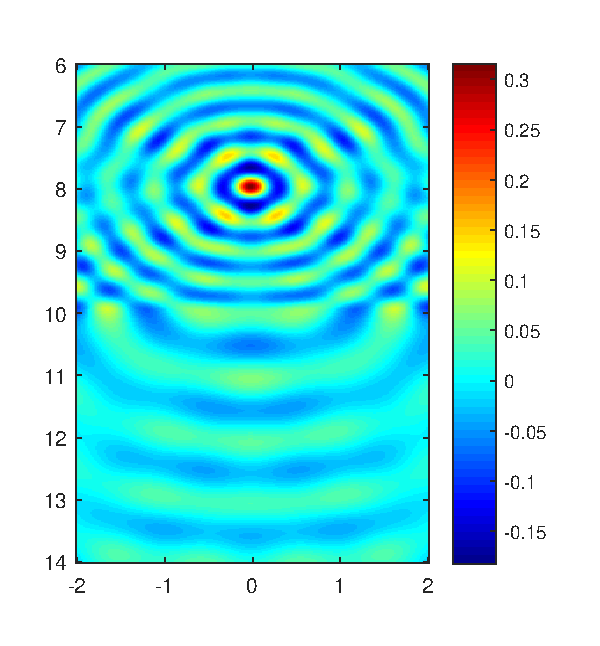
\includegraphics[width=0.4\textwidth]{./half/psf/in_imagesc.eps}
  \includegraphics[width=12cm,height=6cm]{./waveguide1/psf_half/in_mesh.eps}
  \caption{$-\Im J_d(z,y)$,其中$G_{bp}(x,z)=G_{k_1}(x,z)$,源点$y_1\in L_1$.}\label{ImagPSF_half1}
\end{figure}
\begin{figure}[h]
  \centering
%  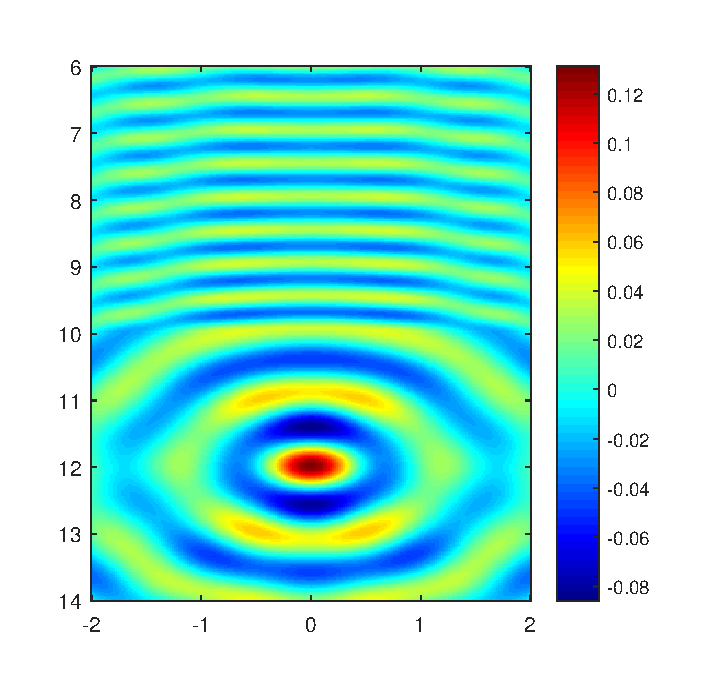
\includegraphics[width=0.4\textwidth]{./half/psf/out_imagesc.eps}
  \includegraphics[width=12cm,height=6cm]{./waveguide1/psf_half/out_mesh.eps}
  \caption{$-\Im J_d(z,y)$,其中$G_{bp}(x,z)=G_{k_1}(x,z)$,源点$y_2\in L_2$.}\label{ImagPSF_half2}
\end{figure}


以上分析表明如果直接将文献\cite{ch_cw,ch_ha}中的想法推广到开波导情形,那么仅仅能够对位于开波导第一层内的障碍物进行有效成像,本章第五小节的数值测试结果也验证了这一事实,而对位于波导第二层的障碍物,选取$G_{k_1}(x,z)$作为反传播函数不再合适。因为在波导第二层波数为$k_2$,反传播函数$G_{k_1}(x,z)$的波数为$k_2$,明显不匹配。另外,由于同样的原因,我们选取$G_{k_2}(x,z)$ 也是不合适的。

\subsection{另一种想法:$G_{bp}(x,z)=G(x,z)$.}
一个比较自然的改进想法是选取$G_{bp}(x,z)=G(x,z)$,其中$G(x,y)$表示源点为$y$ 的Pekeris开波导Dirichlet 零边界格林函数,即
\begin{eqnarray}\label{G_Dirichlet}
\left\{
\begin{array}{lll}
  \Delta_xG(x,y)+k^2(x)G(x,y)=-\delta_z(y),&in&\R^2_+\\
  & &\\
  \left[G(\cdot,y)\right]_{\Gamma_h}=0,\ \ \left[\frac{\partial G(\cdot,y)}{\partial\nu}\right]_{\Gamma_h}=0 & &\\
  & &\\
  G(x,y)=0, &on&\Gamma_0
\end{array}
\right.
\end{eqnarray}
类似于格林函数$N(x,y)$,通过相同的手段,我们可以得到格林函数$G(x,y)$的积分表达式和波导模式展开表达式:
\begin{lemma}\label{f_Dirichlet}
令$\xi=\xi_1+\i\xi_2,\xi_1,\xi_2\in\R$,以及$\mu_j=\sqrt{k_j^2-\xi^2},j=1,2$,并记关于$\xi$的函数$N_h(\xi)$和$M_h(\xi)$如下所示
\begin{eqnarray}\label{NhMh}
 N_h(\xi)=\frac{\mu_1+\mu_2}{\mu_1-\mu_2}+e^{2\i\mu_1h},\ \
 M_h(\xi)=1+\frac{\mu_1+\mu_2}{\mu_1-\mu_2}e^{2\i\mu_1h},
\end{eqnarray}
则方程\ref{G_Dirichlet} 所定义的函数$G(x,y)$有如下表达式
\begin{eqnarray*}
G(x,y)=\left\{
\begin{array}{lll}
  \Phi_{k_1}(x,y)-\Phi_{k_1}(x,y')+S_1(x,y)&, &x\in L_1,y\in L_1\\
 S_2(x,y)&, &x\in L_2,y\in L_1\\
 K_1(x,y)&, &x\in L_1,y\in L_2\\
 \Phi_{k_2}(x,y)+K_2(x,y)&,&x\in L_2,y\in L_2
\end{array}
\right.
\end{eqnarray*}
其中$S_j(x,y),K_j(x,y),j=1,2$ 的表达式为
\begin{eqnarray*}
\left\{
\begin{array}{lll}
  S_1(x,y)&=&\frac{1}{2\pi}\int_{SIP}\frac{-\i}{2\mu_1}\frac{e^{2\i\mu_1h}\left[4\sin{(\mu_1x_2)\sin{(\mu_1y_2)}}\right]}{N_h(\xi)}
  e^{\i(x_1-y_1)\xi}d\xi\\
  & &\\
  S_2(x,y)&=&\frac{1}{2\pi}\int_{SIP}\frac{2e^{\i\mu_1h}\sin{(\mu_1y_2)}}{(\mu_1-\mu_2)N_h(\xi)}e^{\i\mu_2(x_2-h)+\i(x_1-y_1)\xi}d\xi\\
  & &\\
  K_1(x,y)&=&\frac{1}{2\pi}\int_{SIP}\frac{2e^{\i\mu_1h}\sin(\mu_1x_2)}{(\mu_1-\mu_2)N_h(\xi)}e^{\i\mu_2(y_2-h)+\i(x_1-y_1)\xi}d\xi\\
  & &\\
  K_2(x,y)&=&\frac{1}{2\pi}\int_{SIP}\frac{-\i}{2\mu_2}\frac{M_h(\xi)}{N_h(\xi)}e^{\i\mu_2(x_2+y_2-2h)+\i(x_1-y_1)\xi}d\xi
\end{array}
\right.
\end{eqnarray*}
\end{lemma}
\begin{remark}
同样地,格林函数$G(x,y)$ 的Fourier变换会出现极点,也就是函数$N_h(\xi)$ 的零点。直接验证可知,当$\xi\in\{\xi\in\R;|\xi|>k_1,|\xi|<k_2\}$ 时,
$N_h(\xi)\neq0$。于是当$\xi\in\R$时,$N_h(\xi)$ 的零点仅仅分布在区间$[k_2,k_1]$,或区间$[-k_1,-k_2]$上。特别地,$\xi=\pm k_1$是$N_h(\xi)$的零点,但是我们同时注意到当$\xi=\pm k_1$时,$\hat G_y(\xi,x_2)$中对应于$N_h(\xi)$的分子同样为零,并不会给后面的分析带来麻烦。当$\xi=\pm k_2$ 时,
\begin{equation}
  N_h(\xi)=0\ \ \Rightarrow\ \ \cos\left(\sqrt{k_1^2-k_2^2}h\right)=0
\end{equation}
由该方程可解出频率$\omega=\frac{c_1c_2}{\sqrt{c_2^2-c_1^2}}\frac{(n+\frac{1}{2})\pi}{h}$,称为截断频率。一般地,我们假设$\cos\left(\sqrt{k_1^2-k_2^2}h\right)\neq0$ 以保证模型不会产生截断频率。当$\xi\in(k_2,k_1)$ 时,$N_h(\xi)=0$等价于
\begin{equation}
  \tan{\left(\sqrt{k_1^2-\xi^2}h\right)}=-\frac{\sqrt{k_1^2-\xi^2}}{\sqrt{\xi^2-k_2^2}}
\end{equation}
记$N_h(\xi)$在区间$(k_2,k_1)$上的零点个数为$M$, 则由上式可知,$M\leq\left[\sqrt{k_1^2-k_2^2}h/\pi\right]$。 我们记这$M$个零点为$\xi_1,\ldots,\xi_M$,易验证$N'_h(\xi_m)\neq0$,于是这$M$个零点都是$N_h(\xi)$的一阶零点,它们对应了函数$G(x,y)$的$M$ 个波导模式。

\end{remark}
\begin{lemma}[关于$G(x,y)$的波导模式展开]\label{Dirichlet_Mode}
设$\xi_m$, $m=1,\ldots,M$是函数$N_h(\xi)$在区间$(k_2,k_1)$ 上的$M$ 个实根,并记$\mu_{1m}=\mu_1(\xi_m),\mu_{2m}=\mu_2(\xi_m)$,则$G(x,y)$ 的波导模式展开为
\begin{equation*}
  G(x,y)=G_g(x,y)+G_{rad}(x,y)
\end{equation*}
其中$G_g(x,y)=\sum\limits_{m=1}^M G_m(x,y)$,且
\begin{eqnarray}
\left\{
\begin{array}{lll}
  G_m(x,y)&=&\frac{\mu_{2m}}{\xi_m(1-\i\mu_{2m}h)}g(x_2,\xi_m)g(y_2,\xi_m)e^{\i|x_1-y_1|\xi_m}\\
& &\\
 G_{rad}(x,y)&=&\frac{\ii}{\pi}\int_{\ii\infty}^{k_2}\frac{\mu_2 g(x_2,\xi)g(y_2,\xi)}{(k_1^2-k_2^2)\cos^2(\mu_1h)+\mu_2^2}e^{\ii|x_1-y_1|\xi}d\xi
\end{array}
\right.
\end{eqnarray}
其中$G_m(x,y)$中对应于$\xi_m\in(k_2,k_1)$的$g(x_2,\xi_m)$ 表达式如下
 \begin{eqnarray*}
 g(x_2,\xi_m):=\left\{
 \begin{array}{lll}
   \sin(\mu_{1m}x_2),& &x_2\in(0,h)\\
   & &\\
   \sin(\mu_{1m}h)e^{\i\mu_{2m}(x_2-h)},& &x_2\in(h,+\infty)
 \end{array}
 \right.
 \end{eqnarray*}
此外$G_{rad}(x,y)$中有向积分区间$[\i\infty,k_2]:=\{\xi;\xi\in[0,k_2],\ \ \mbox{或}\xi=\i\eta$,$\eta\in(0,+\infty)\}$,以及对应于$\xi\in[\i\infty,k_2]$的函数$g(x_2,\xi)$ 如下
 \begin{eqnarray*}
 g(x_2,\xi):=\left\{
 \begin{array}{lll}
   \sin(\mu_1x_2),& &x_2\in(0,h)\\
   & &\\
   \sin(\mu_1h)\cos[\mu_2(x_2-h)]+\frac{\mu_1}{\mu_2}\cos(\mu_1h)\sin[\mu_2(x_2-h)],& &x_2\in(h,+\infty)
 \end{array}
 \right.
 \end{eqnarray*}
\end{lemma}


我们期待选取$G(x,z)$为反传播函数可以解决之前遇到的波数不一致问题,数值测试结果也间接表明这种方法或许可取。设定测试参数与之前完全一样,测试结果如图\ref{ImagPSF_wg1}和\ref{ImagPSF_wg2}所示。从测试结果来看,选取函数$G(x,z)$ 作为反传播函数能够很好地解决问题\ref{pro_psf}。
\begin{figure}[h]
  \centering
%  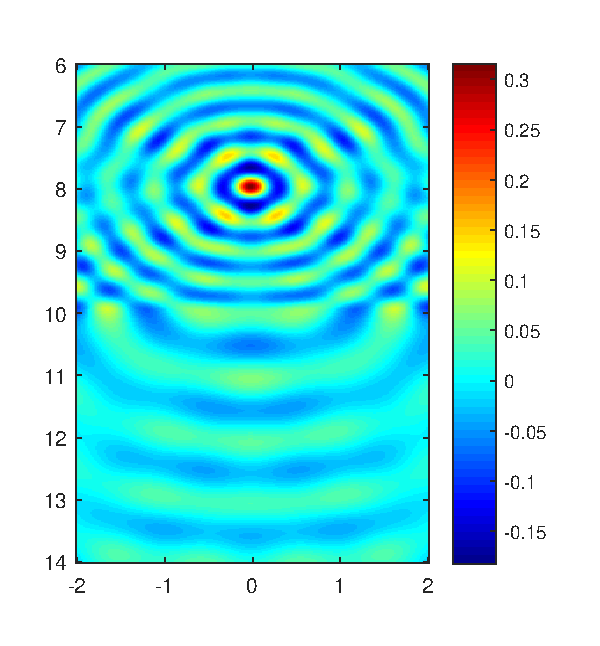
\includegraphics[width=0.4\textwidth]{./half/psf/in_imagesc.eps}
  \includegraphics[width=13cm,height=5cm]{./waveguide1/psf_waveguide/in_mesh.eps}
  \caption{$-\Im J_d(z,y)$,其中$G_{bp}(x,z)=G(x,z)$,源点$y_1\in L_1$.}\label{ImagPSF_wg1}
\end{figure}
\begin{figure}[h]
  \centering
%  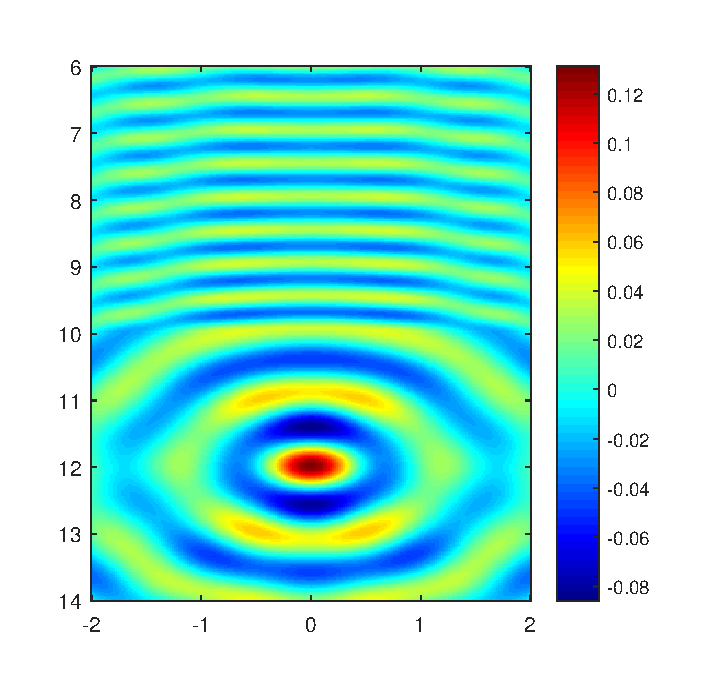
\includegraphics[width=0.4\textwidth]{./half/psf/out_imagesc.eps}
  \includegraphics[width=13cm,height=5cm]{./waveguide1/psf_waveguide/out_mesh.eps}
  \caption{$-\Im J_d(z,y)$,其中$G_{bp}(x,z)=G(x,z)$,源点$y_2\in L_2$.}\label{ImagPSF_wg2}
\end{figure}
\section{Pekeris开波导逆时偏移算法}
通过对点扩散函数的分析和测试,我们提出针对Pekeris开波导障碍物成像问题的逆时偏移算法:
\begin{algorithm}\label{alg_wg}
设$\Omega$为采样区域,令$u^s(x_r,x_s)$ 为在接收点$x_r$收到的由源点$x_s$ 所激发的散射数据,其中$x_r,x_s\in\Gamma_0^d;r=1,\ldots,N_r;s=1,\ldots,N_s$.\\
$1^\circ$ 反传播: 对$s=1,\ldots,N_s$,计算反传播场
\begin{equation}
  v_b(z,x_s)=\frac{|\Gamma_0^d|}{N_r}\sum\limits_{r=1}^{N_r}\frac{\partial G(x_r,z)}{\partial x_2(x_r)}\overline{u^s(x_r,x_s)},\  \  \forall z\in\Omega.
\end{equation}
若令$N_r\rightarrow0$,则上式可看做如下积分的数值近似,
\begin{equation}
  \hat v_b(z,x_s)=\int_{\Gamma_0^d}\frac{\partial G(x_r,z)}{\partial x_2(x_r)}\overline{u^s(x_r,x_s)}ds(x_r)
\end{equation}
$2^\circ$ 互相关: 对$z\in\Omega$,计算成像函数
\begin{equation}
  I_d(z)=\Im\left\{\frac{|\Gamma_0^d|}{N_s}\sum\limits_{s=1}^{N_s}\frac{\partial G(x_s,z)}{\partial x_2(x_s)}v_b(z,x_s)
  \right\}.
\end{equation}
将$v_b(z,x_s)$的表达式代入$I_d(z)$,可得
\begin{equation}\label{Id_wg}
  I_d(z)=\Im\left\{\frac{|\Gamma_0^d|}{N_s}\frac{|\Gamma_0^d|}{N_r}\sum\limits_{s=1}^{N_s}\sum\limits_{r=1}^{N_r}\frac{\partial G(x_s,z)}{\partial x_2(x_s)}\frac{\partial G(x_r,z)}{\partial x_2(x_r)}\overline{u^s(x_r,x_s)}
  \right\}.
\end{equation}
成像函数\eqref{Id_wg} 将用于下节所有的数值算例测试。
若令$N_s,N_r\rightarrow\infty$,则上式可看做如下积分的数值近似,
\begin{equation}\label{Id_wg_hat}
  \hat I_d(z)=\Im\int_{\Gamma_0^d}\int_{\Gamma_0^d}\frac{\partial G(x_s,z)}{\partial x_2(x_s)}
  \frac{\partial G(x_r,z)}{\partial x_2(x_r)}\overline{u^s(x_r,x_s)}ds(x_r)ds(x_s).
\end{equation}
\end{algorithm}

\section{数值测试}

在本小节我们将通过数值算例来测试算法\ref{alg_wg} 对嵌入在开波导结构中障碍物的成像效果。 散射数据$u^s(x_r,x_s)$ 由标准的Nystr\"om 方法生成。在求解边界$\Gamma_D$上的积分方程时,我们每个波长布置10个离散点。本章主要依旧采用如下具有参数表示的障碍物边界作为测试算例,分别为$P$叶风扇形状、 圆形、花生形状以及边角被光滑后的方块形状,它们的参数表达分别如下
\begin{eqnarray}\label{obstacle_example2}
\left\{
\begin{array}{lll}
x_1=r(\theta)\cos\theta&,& x_2=r(\theta)\sin\theta,\ \ \mbox{其中}\ \ r(\theta)=1+0.2\cos(p\theta),\\
x_1=\rho\cos{\theta}&,& x_2=\rho\sin{\theta},\\
x_1=\cos{\theta}+0.2\cos{3\theta}&,& x_2=\sin{\theta}+0.2\sin{3\theta},\\
x_1=\cos^3\theta+\cos{\theta}&,& x_2=\sin^3\theta+\sin{\theta}.
\end{array}
\right.
\end{eqnarray}
\subsection{障碍物$D\subset L_1$.}
在本小节中,我们先考虑障碍物位于Pekeris开波导第一层$L_1$,即假设$D\subset L_1$。 我们令$h=10,d=50$,且源点$x_s$ 和接收点$x_r$ 在$\Gamma_0^d$ 上均匀分布,其中$\Gamma_0^d=\{(x_1,x_2)\in\R^2;x_1\in(-d,d),x_2=0\}$。 采样区域为$\Omega=[-2,2]\times[6,10]$,且我们采用$201\times201$ 的均匀采样。探测频率为$k_1=4\pi,k_2=2\pi$。 源点和接收点个数为$N_s=256,N_r=256$。
\begin{example}[不同形状]\label{wg_ex1}
在本算例中,我们以声软障碍物为例测试位于Pekeris 开波导第一层具有不同形状的障碍物,例如4叶风扇形状,矩形形状,花生形状和椭圆形状,算法\ref{alg_wg}的成像效果。与此同时,我们也同时测试当所采用的反传播函数为$G_{k_1}(x,z)$ 时,即如下成像函数:
\begin{equation}\label{Id_half}
   I_d^{k_1}(z)=\Im\left\{\frac{|\Gamma_0^d|}{N_s}\frac{|\Gamma_0^d|}{N_r}\sum\limits_{s=1}^{N_s}\sum\limits_{r=1}^{N_r}\frac{\partial G_{k_1}(x_s,z)}{\partial x_2(x_s)}\frac{\partial G_{k_1}(x_r,z)}{\partial x_2(x_r)}\overline{u^s(x_r,x_s)}
  \right\}.
\end{equation}
的成像效果。

测试结果如图\ref{fig_wg_ex1}所示,当障碍物位于Pekeris开波导第一层$L_1$时,两种成像函数都能够对不同形状的声软障碍物做到有效成像。除此之外,通过对比,我们可以看到:在相同参数下,算法\ref{alg_wg}的成像函数\eqref{Id_wg}的成像效果要远远好于采用函数$G_{k_1}(x,z)$作为反传播函数时所对应的成像函数\eqref{Id_half}。事实上,成像函数\ref{Id_wg}的成像值几乎都是正值,具有更好的稳定性,而且其不仅仅确定了声软障碍物的上边界,对于下边界以及侧边界也可以做到稍微粗浅的成像。
\end{example}

\begin{figure}[h]
  \centering
  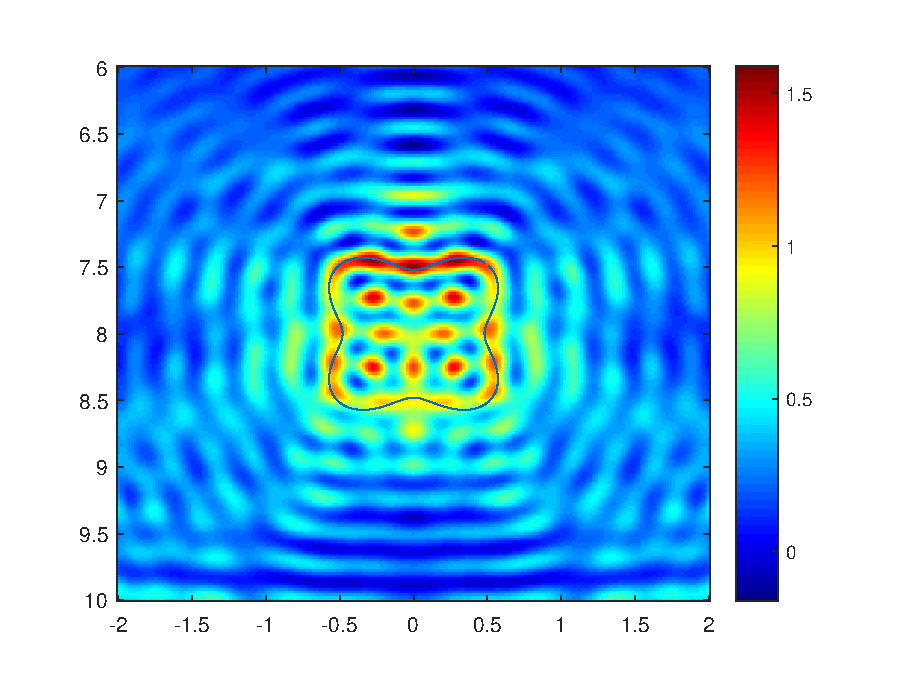
\includegraphics[width=0.23\textwidth]{./waveguide1/example1/In_soft_pleaf1.eps}
  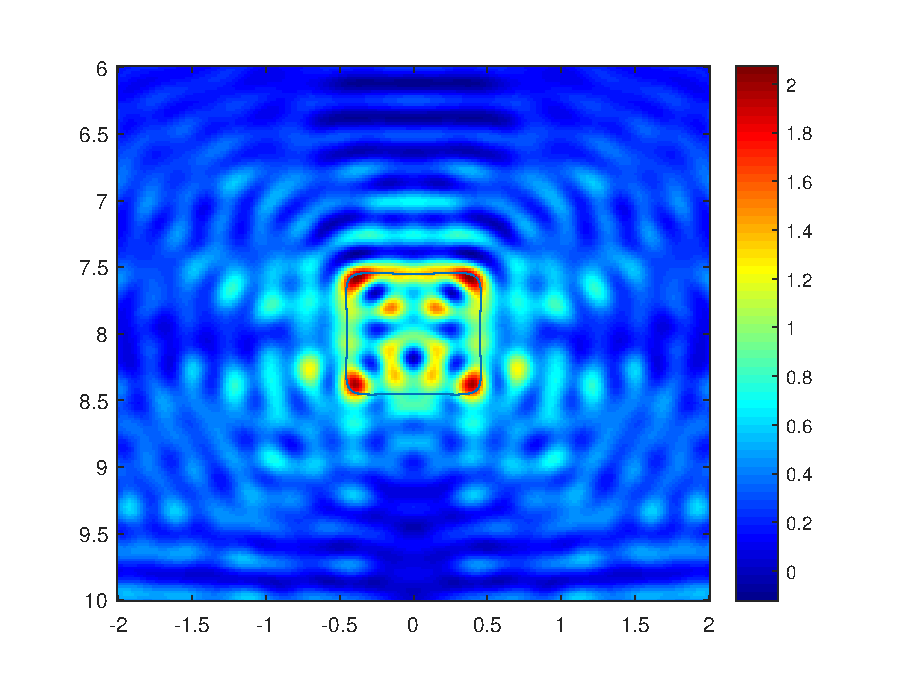
\includegraphics[width=0.23\textwidth]{./waveguide1/example1/In_soft_square1.eps}
  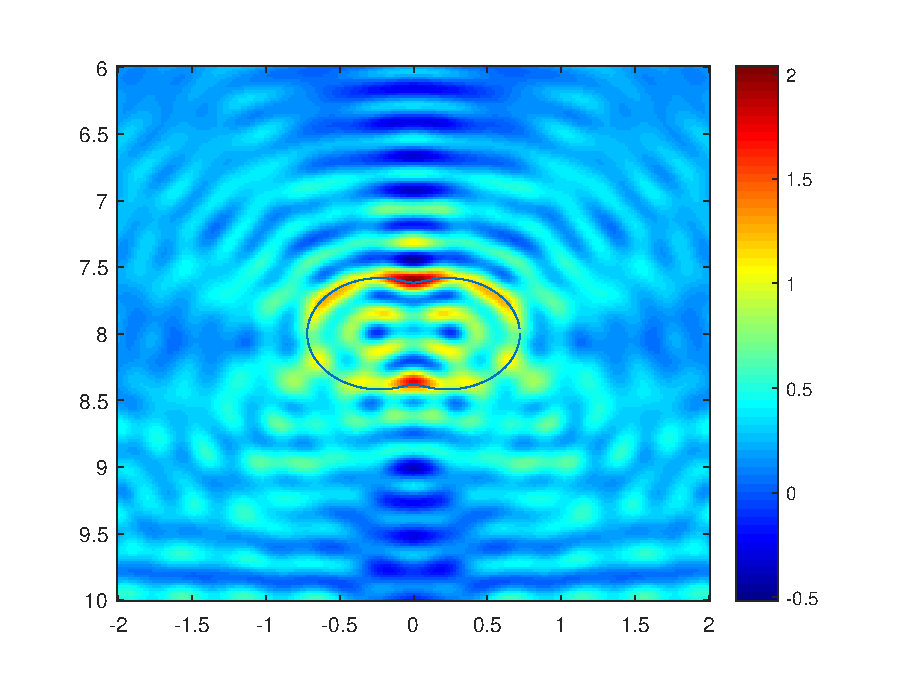
\includegraphics[width=0.23\textwidth]{./waveguide1/example1/In_soft_peanut.eps}
  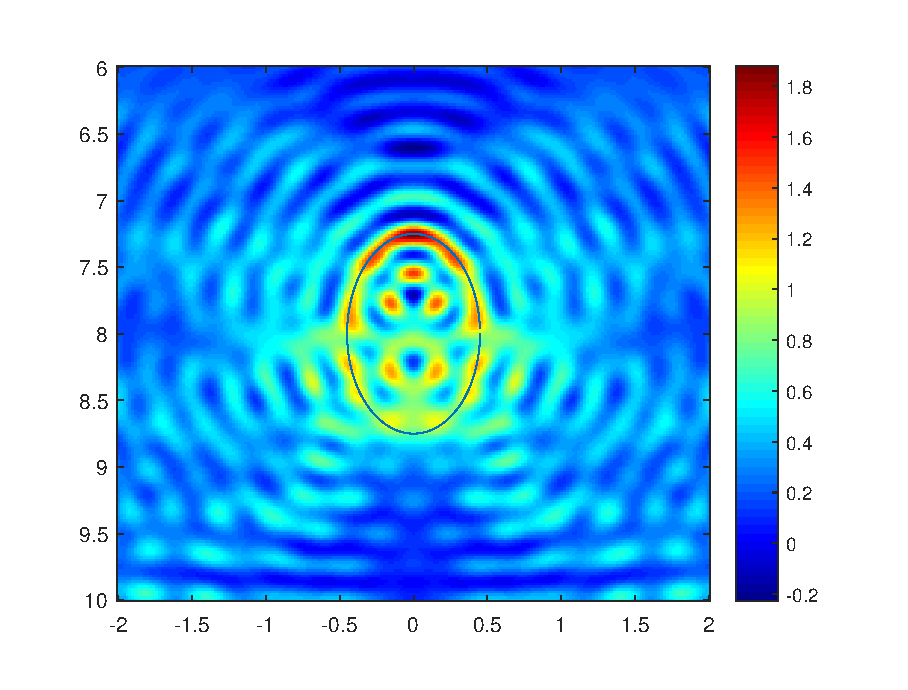
\includegraphics[width=0.23\textwidth]{./waveguide1/example1/In_soft_circle1.eps}
  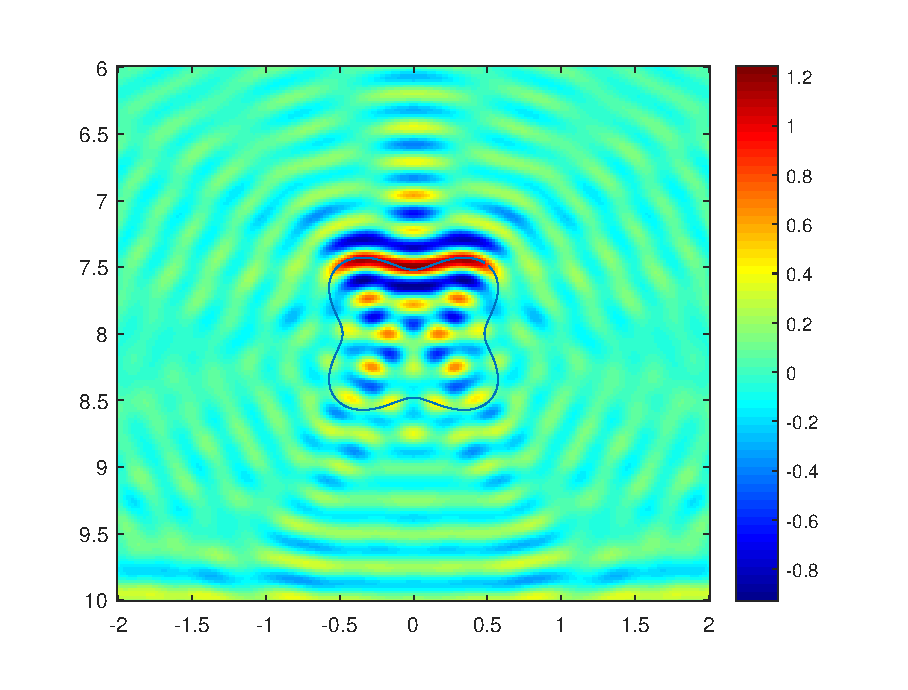
\includegraphics[width=0.23\textwidth]{./waveguide1/example1/In_soft_pleaf1_half.eps}
  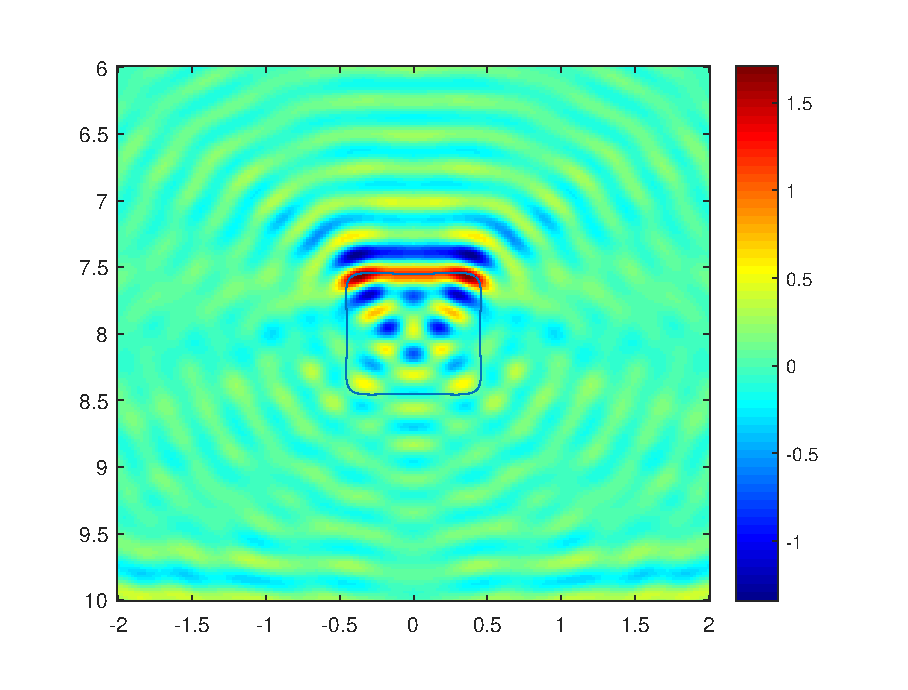
\includegraphics[width=0.23\textwidth]{./waveguide1/example1/In_soft_square1_half.eps}
  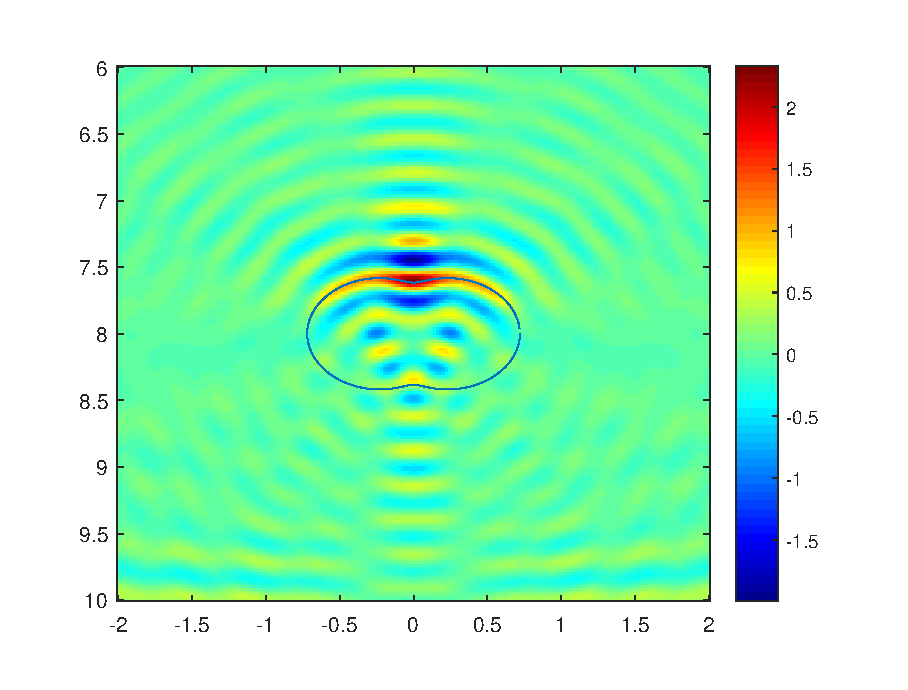
\includegraphics[width=0.23\textwidth]{./waveguide1/example1/In_soft_peanut_half.eps}
  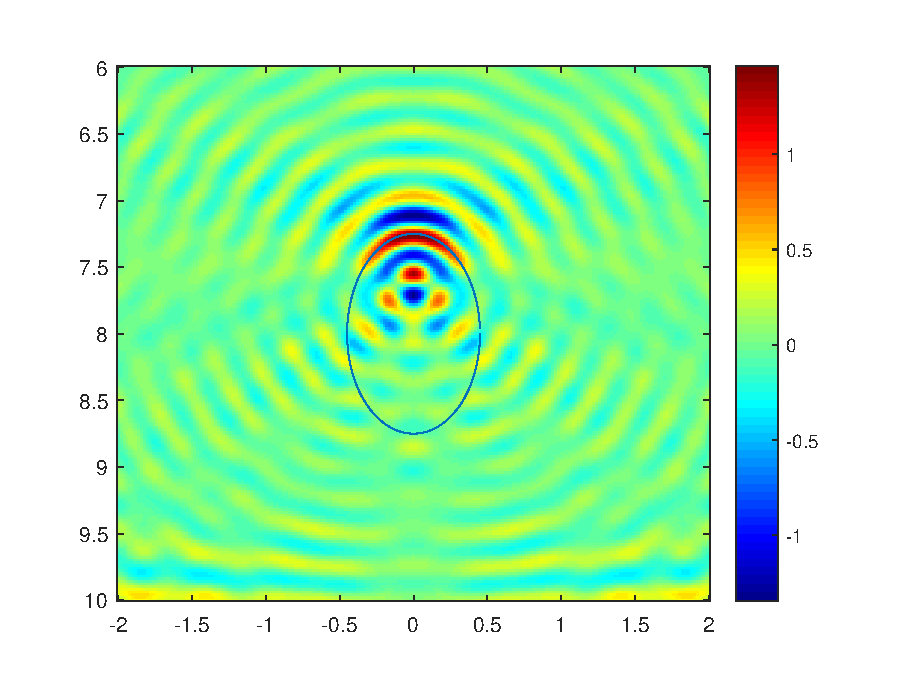
\includegraphics[width=0.23\textwidth]{./waveguide1/example1/In_soft_circle1_half.eps}
  \caption{算例\ref{wg_ex1}:测试不同形状的声软障碍物成像效果,从左到右依次为4 叶风扇、矩形、花生以及椭圆形状,其中第一行为算法\ref{alg_wg}成像函数\ref{Id_wg}的成像效果,第二行为反传播函数是函数$G_{k_1}(x,z)$时所对应成像函数\ref{Id_half}的成像效果。}\label{fig_wg_ex1}
\end{figure}

\begin{example}[不同边界类型]\label{wg_ex2}
在本算例中,我们以圆形障碍物为例,验证算法\ref{alg_wg}对位于Pekeris 开波导第一层具有不同边界类型的障碍物的成像效果。例如声软障碍物,声硬障碍物,折射系数为$n(x)$ 的可穿透障碍物,阻尼系数为$\eta(x)$的阻抗边界障碍物。对于可穿透障碍物成像,我们假设折射系数$n(x)$ 为:
\begin{eqnarray*}
n(x)=\left\{
\begin{array}{lll}
  0.5&,&x\in D\\
  1&,&x\in\R_+^2\backslash\overline D
\end{array}
\right.
\end{eqnarray*}
对于阻抗边界障碍物,我们假设在上半边界$\eta(x)=1$,在下半边界$\eta(x)=2$。

数值测试结果如图\ref{fig_wg_ex2}所示,结果表明:在不知道障碍物的任何先验信息的情况下,如是否可穿透,以及不可穿透障碍物的边界条件,两种成像函数都能够对不同类型的圆形障碍物做到有效成像。类似地,算法\ref{alg_wg}所对应成像函数\eqref{Id_wg}的成像效果依旧远远好于当反传播函数为$G_{k_1}(x,z)$时所对应成像函数\eqref{Id_half}的成像效果。从图\ref{fig_wg_ex2}第四列的对比可以看出,即使障碍物为可穿透类型时,成像函数\eqref{Id_wg}也明显优于\eqref{Id_half},因为其不仅能对上下边界进行成像,而且对于侧边界也有不错的成像效果。
\end{example}
\begin{figure}[htbp]
  \centering
  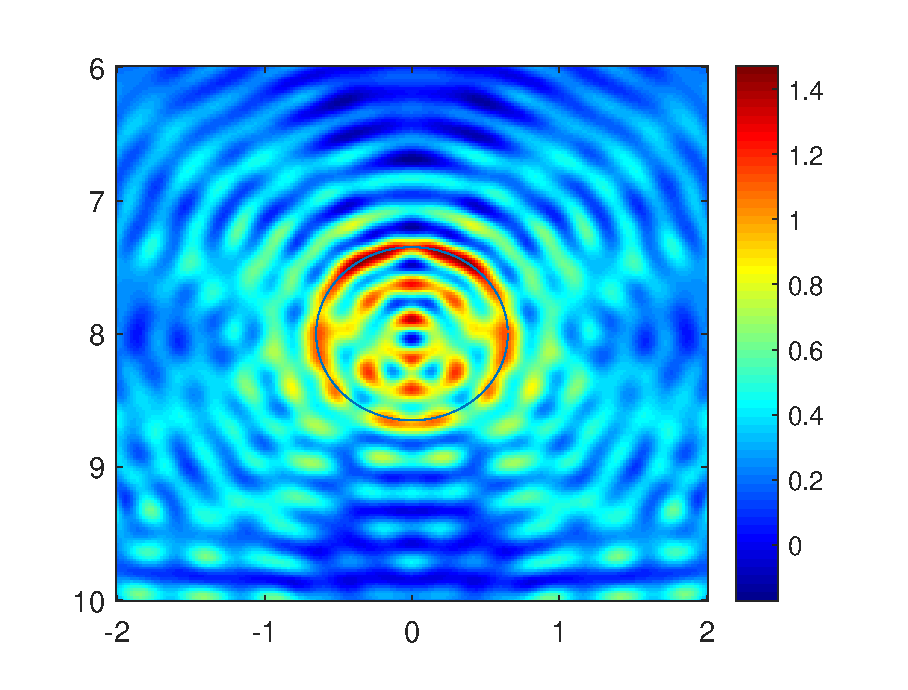
\includegraphics[width=0.23\textwidth]{./waveguide1/example2/In_Circle_Soft.eps}
  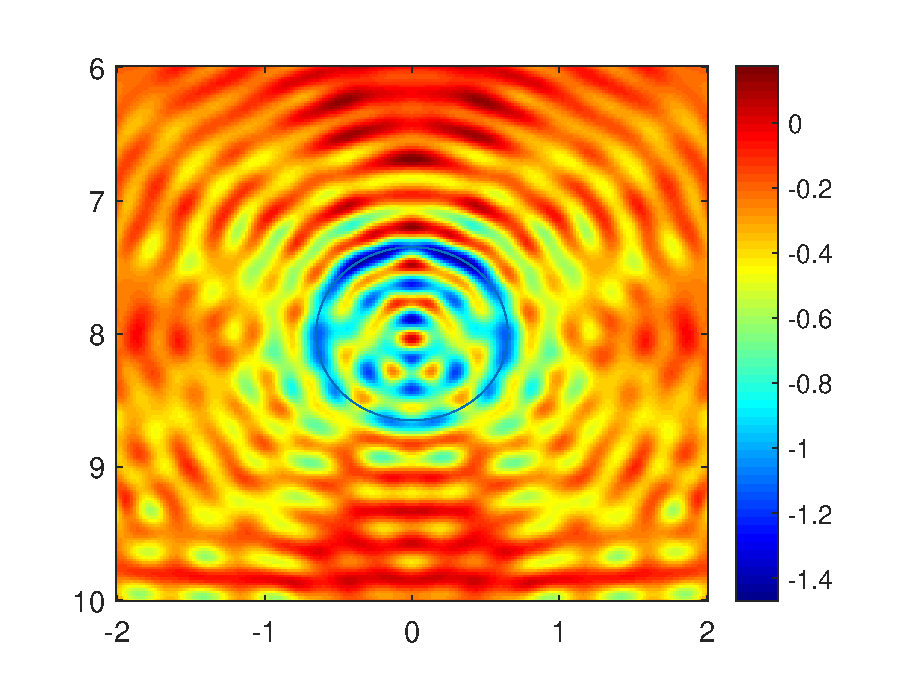
\includegraphics[width=0.23\textwidth]{./waveguide1/example2/In_Circle_Hard.eps}
  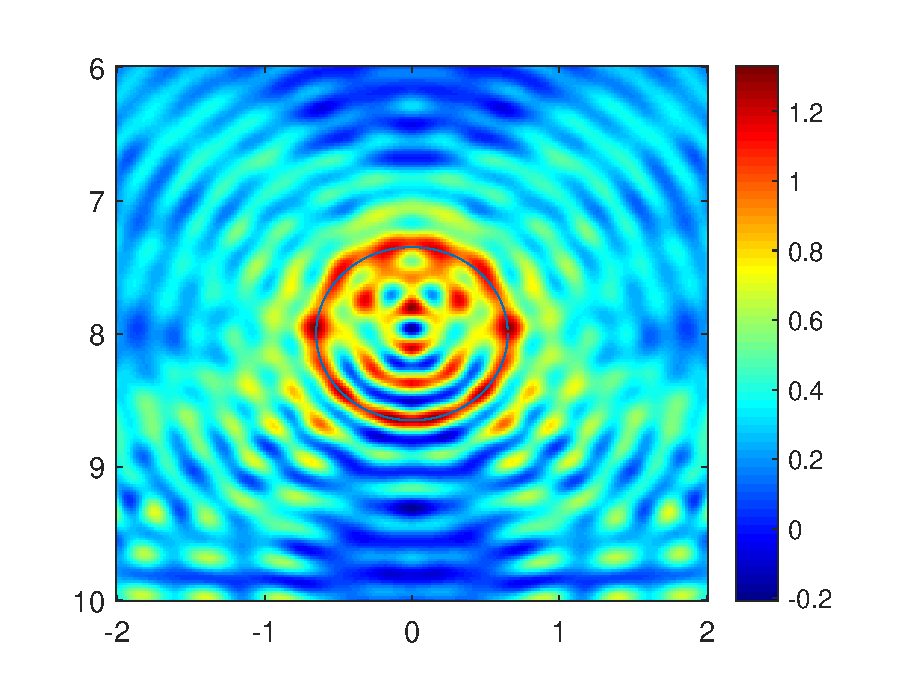
\includegraphics[width=0.23\textwidth]{./waveguide1/example2/In_Circle_Imp.eps}
  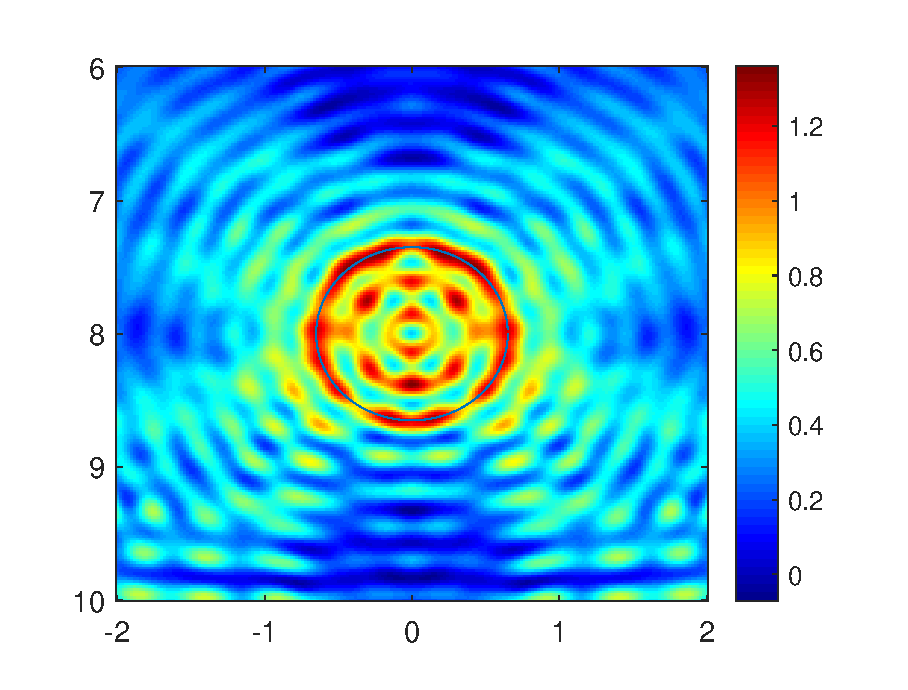
\includegraphics[width=0.23\textwidth]{./waveguide1/example2/In_Circle_Tran.eps}
  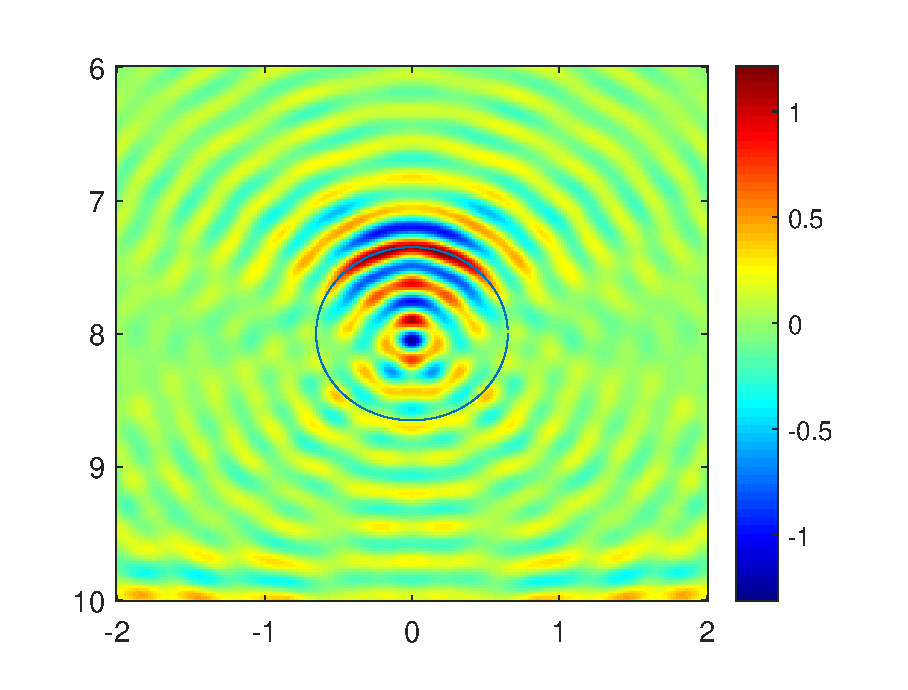
\includegraphics[width=0.23\textwidth]{./waveguide1/example2/In_Circle_Soft_half.eps}
  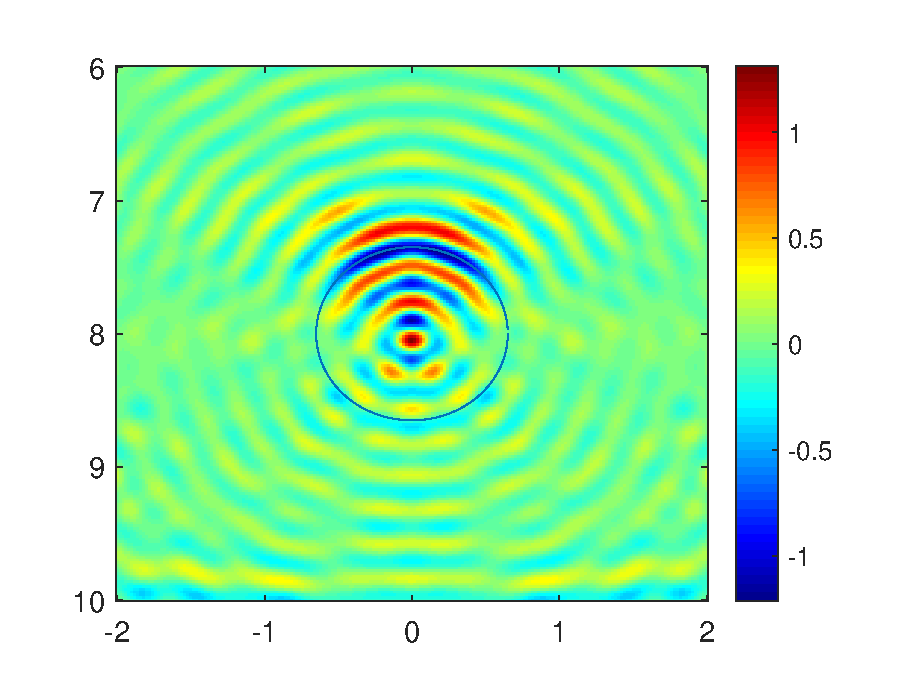
\includegraphics[width=0.23\textwidth]{./waveguide1/example2/In_Circle_Hard_half.eps}
  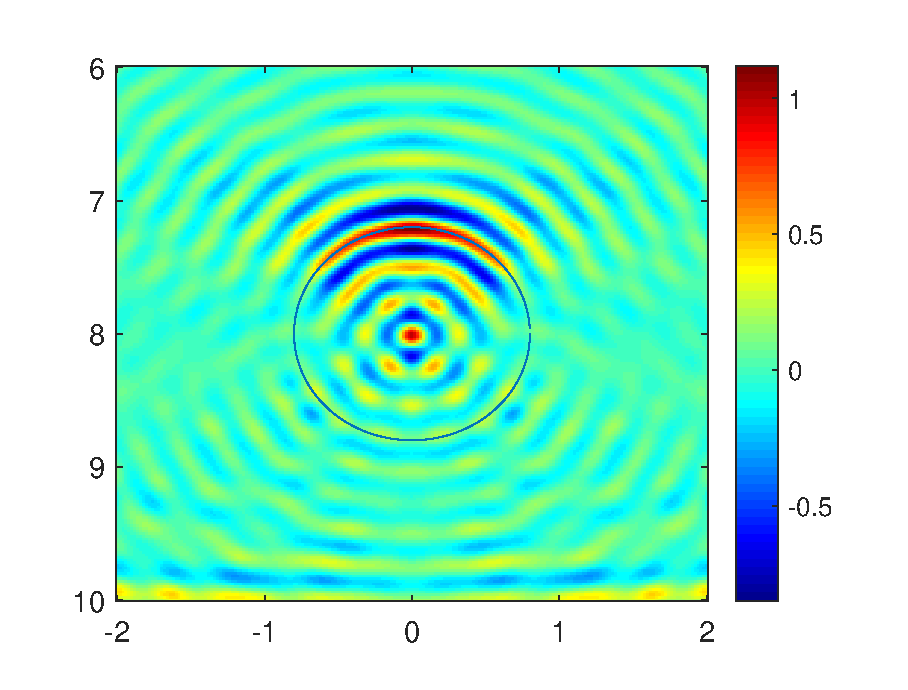
\includegraphics[width=0.23\textwidth]{./waveguide1/example2/In_Circle_Imp_half.eps}
  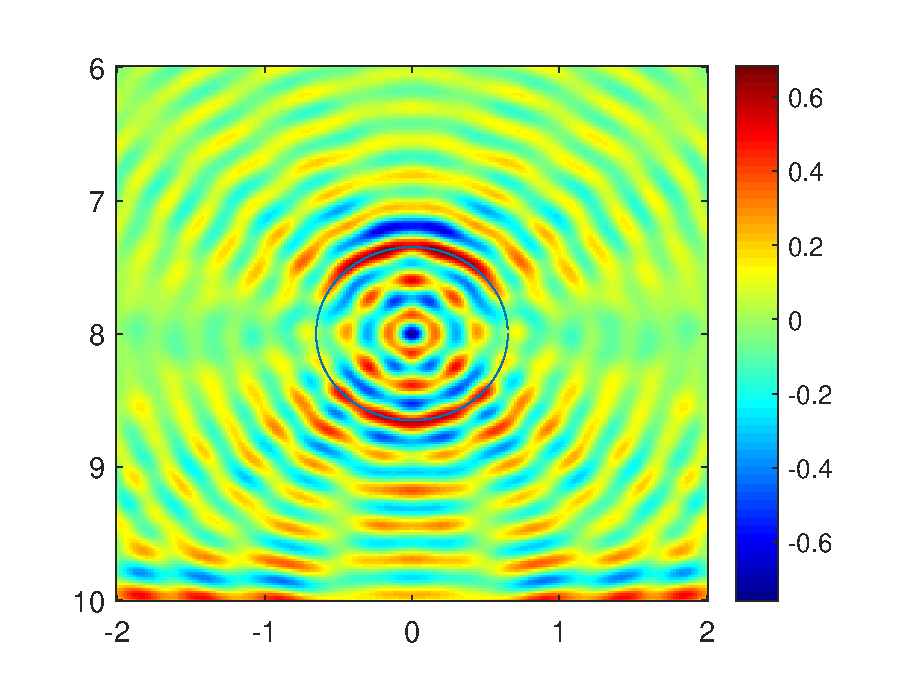
\includegraphics[width=0.23\textwidth]{./waveguide1/example2/In_Circle_Tran_half.eps}
  \caption{算例\ref{wg_ex2}:测试不同类型不同边界的障碍物:前面三个从左到右依次为声软障碍物、声硬障碍物、阻尼系数为$\eta(x)$的阻抗边界障碍物,最后一个为折射系数为$n(x)$的可穿透障碍物,其中第一行为算法\ref{alg_wg}成像函数\ref{Id_wg}的成像效果,第二行为反传播函数是函数$G_{k_1}(x,z)$时所对应成像函数\ref{Id_half}的成像效果。}\label{fig_wg_ex2}
\end{figure}


\begin{example}[抗噪性测试]\label{wg_ex3}
在本算例中,我们测试当在$\Gamma_0^d$上做采集到的散射数据$u^s(x_r,x_s)$带有噪音时,对嵌入在Pekeris开波导第一层$L_1$的障碍物$D$,算法\ref{alg_wg}的成像函数\eqref{Id_wg}的抗噪性能。一般地,我们假设$u^s_{noise}(x_r,x_s)$ 为如下带有高斯噪音的散射数据:
$$ u^s_{noise}(x_r,x_s)=u^s(x_r,x_s)+v_{noise},$$
其中$v_{noise}$为满足如下分布的高斯噪音:
$$v_{noise}=\mu \max{|u^s|}\epsilon,\ \ \epsilon\sim N(0,1).$$

我们第一个测试的是4-叶风扇形状的声软障碍物,测试结果如图\ref{fig_wg_ex3_1}所示:假设从左到右噪音水平$\mu$按如下数值依次递增:$0.1,0.2,0.4,0.6$,其中第一行为单频测试结果,测试频率为$k_1=4\pi,k_2=2\pi$;第二行为多频测试结果,测试频率为$k_2=\frac{1}{2}k_1,k_1=2\pi+0.4n\pi,n=0,1\ldots,9$。结果表明:算法\ref{alg_wg}中的成像函数\ref{Id_wg}具有十分良好的抗噪性能;此外,当采集到的数据为多个频率时,将多个频率的成像函数直接进行相加,能够很好地改善成像效果,大大提高对噪音的抵抗能力;最后多频测试结果还表明算法\ref{alg_wg}在确定所探寻的障碍物的位置时是十分准确而不带偏差的。

我们第二个测试的是圆形的折射系数$n(x)$为
\begin{eqnarray*}
	n(x)=\left\{
	\begin{array}{lll}
		0.5&,&x\in D\\
		1&,&x\in\R_+^2\backslash\overline D
	\end{array}
	\right.
\end{eqnarray*}
的可穿透障碍物,测试结果如图\ref{fig_wg_ex3_2}所示:噪音水平和测试频率的设置与上一个测试算例一模一样,第一、二行分别为单频和多频测试结果。测试结果表明:多频能够极大提高算法\ref{alg_wg}的抗噪音性能;此外,对于可穿透障碍物而言,算法的成像效果要优于不可穿透障碍物,如声软障碍物,这也是符合预期的。
\end{example}
\begin{figure}[htbp]
  \centering
  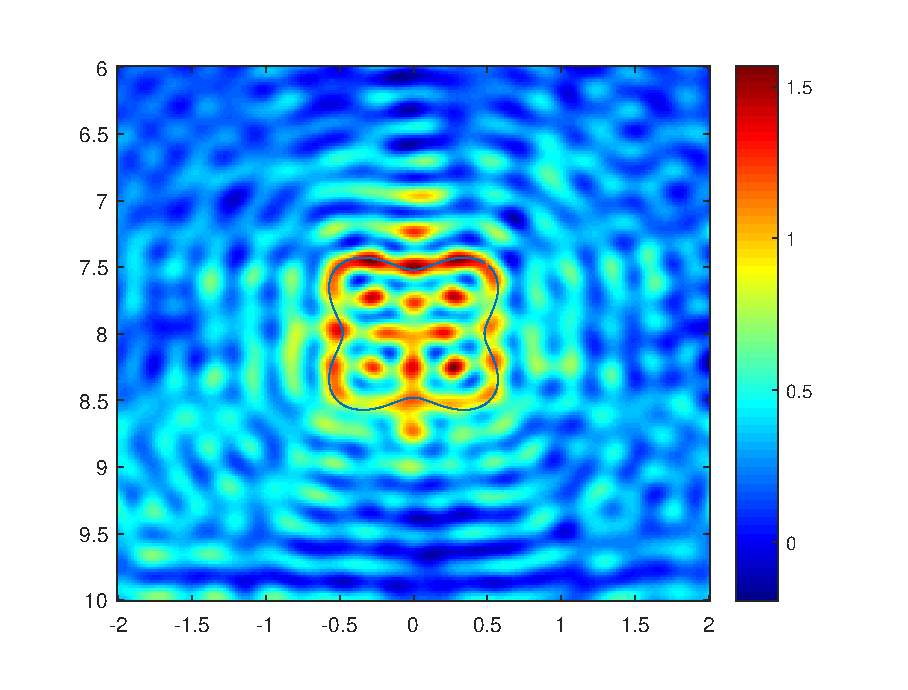
\includegraphics[width=0.23\textwidth]{./waveguide1/example3/In_soft_pleaf1_2.eps}
  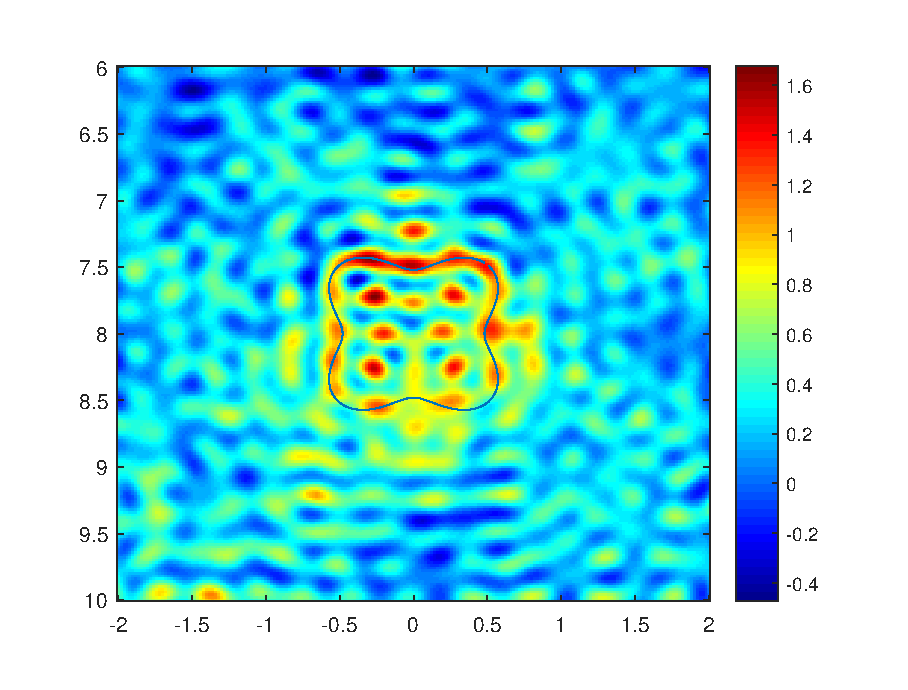
\includegraphics[width=0.23\textwidth]{./waveguide1/example3/In_soft_pleaf1_4.eps}
  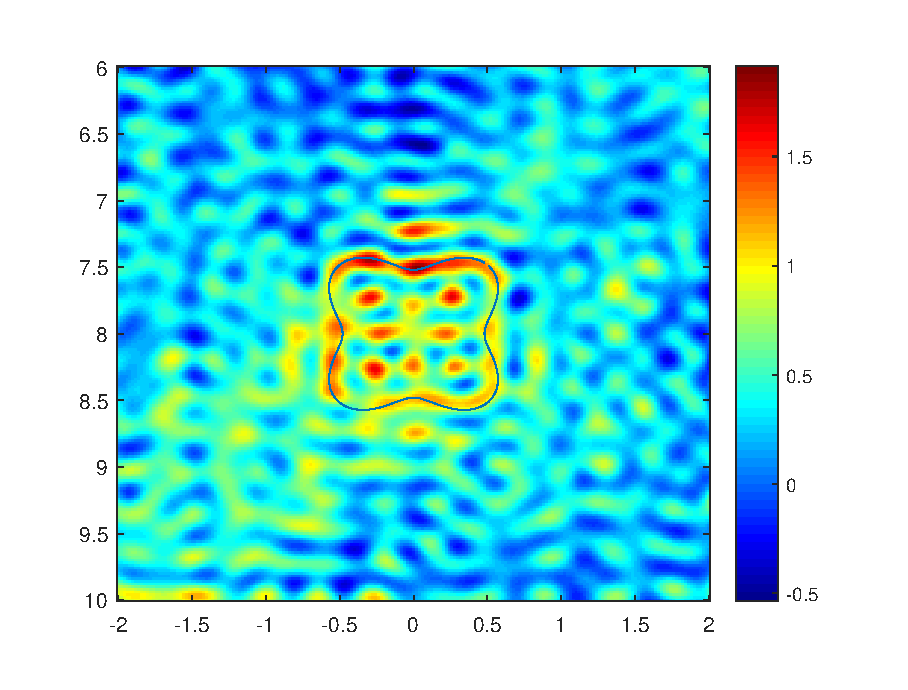
\includegraphics[width=0.23\textwidth]{./waveguide1/example3/In_soft_pleaf1_5.eps}
  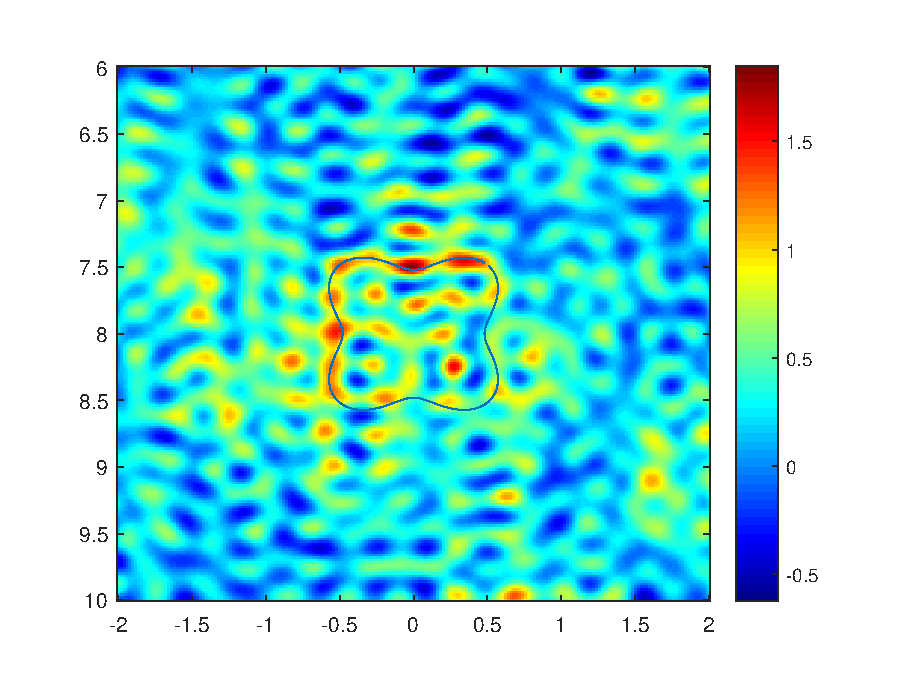
\includegraphics[width=0.23\textwidth]{./waveguide1/example3/In_soft_pleaf1_6.eps}
  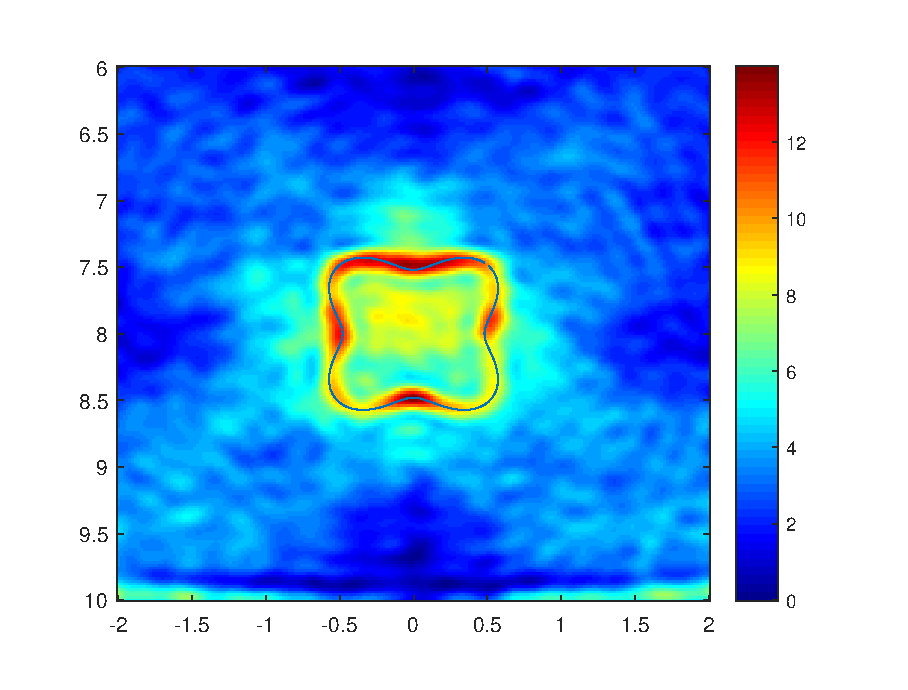
\includegraphics[width=0.23\textwidth]{./waveguide1/example3/In_soft_pleaf1_4_multi.eps}
  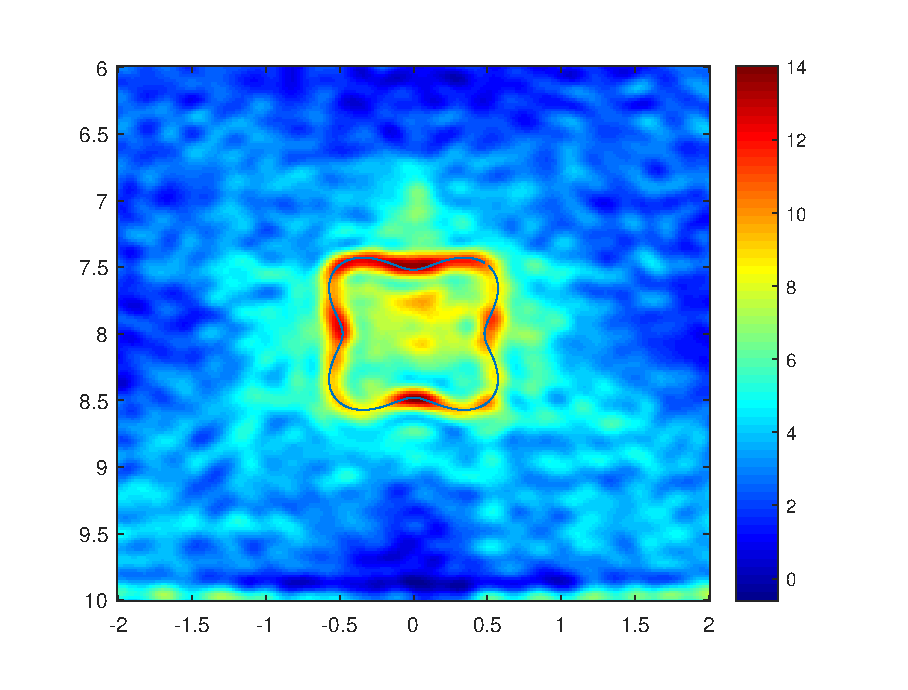
\includegraphics[width=0.23\textwidth]{./waveguide1/example3/In_soft_pleaf1_6_multi.eps}
  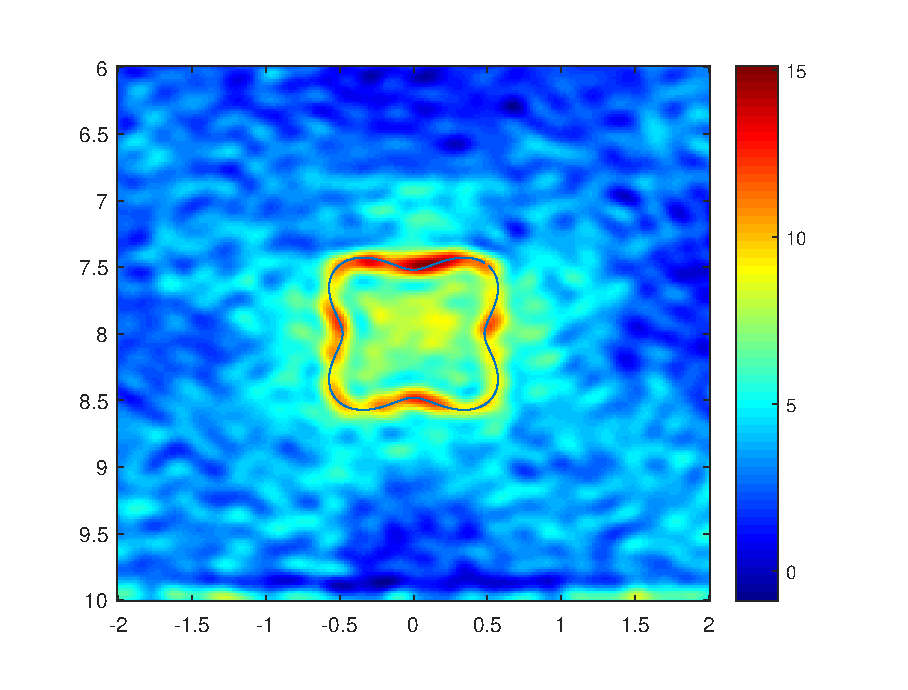
\includegraphics[width=0.23\textwidth]{./waveguide1/example3/In_soft_pleaf1_8_multi.eps}
  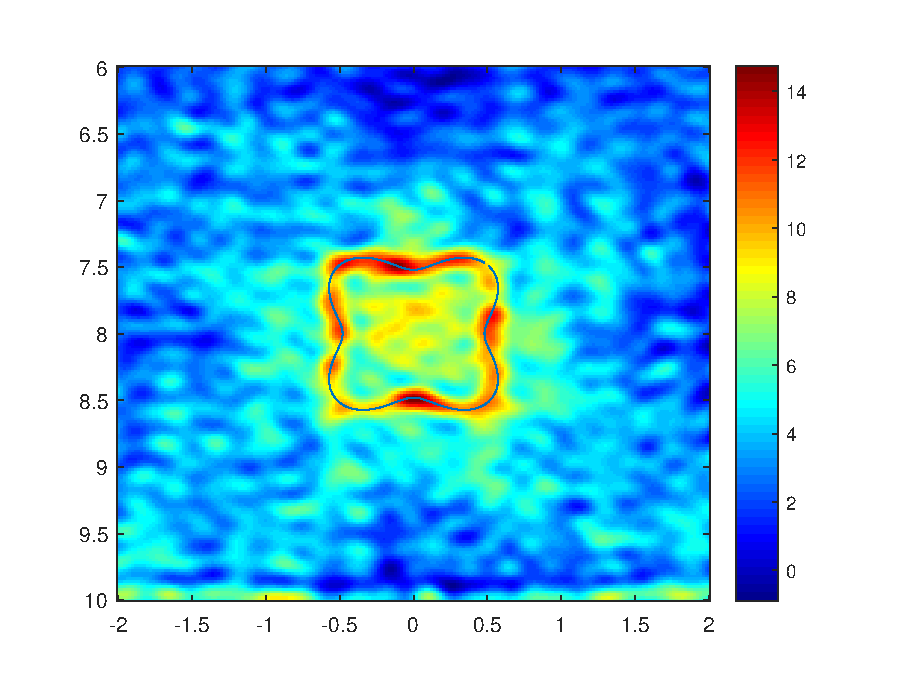
\includegraphics[width=0.23\textwidth]{./waveguide1/example3/In_soft_pleaf1_10_multi.eps}
  \caption{算例\ref{wg_ex3}:测试算法\ref{alg_wg}的抗噪音性能:目标障碍物为4-叶风扇形声软障碍物,噪音水平$\mu$从左到右按如下数值依次递增:$0.1,0.2,0.4,0.6$。其中第一行为单频测试结果,测试频率为:$k_1=4\pi,k_2=2\pi$;第二行为多频测试结果,测试频率为:$k_2=\frac{1}{2}k_1,k_1=2\pi+0.4n\pi,n=0,1\ldots,9$。}\label{fig_wg_ex3_1}
\end{figure}
\begin{figure}[htbp]
  \centering
  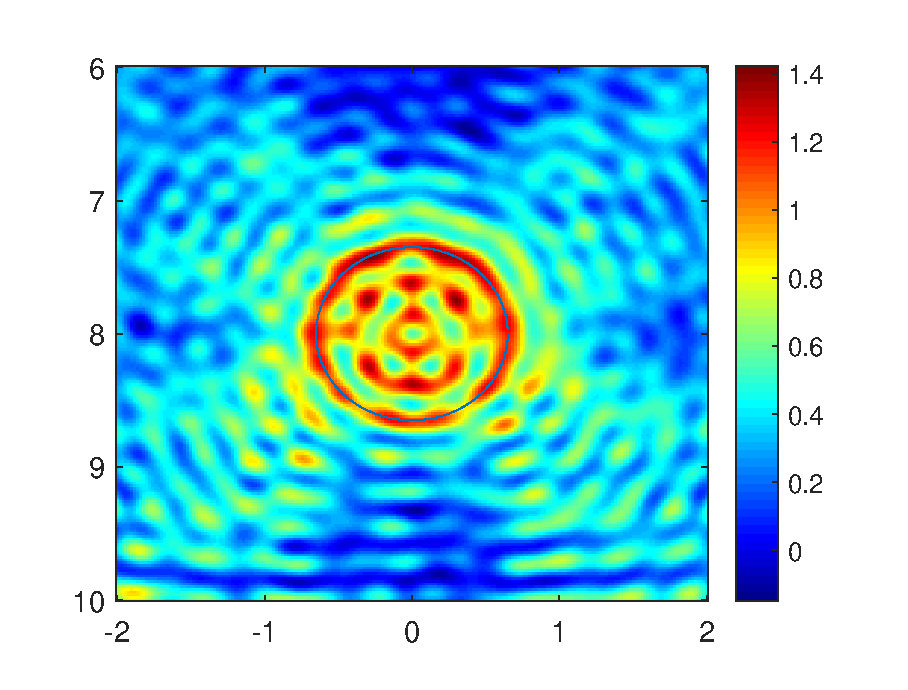
\includegraphics[width=0.23\textwidth]{./waveguide1/example3/In_transmission_circle_2.eps}
  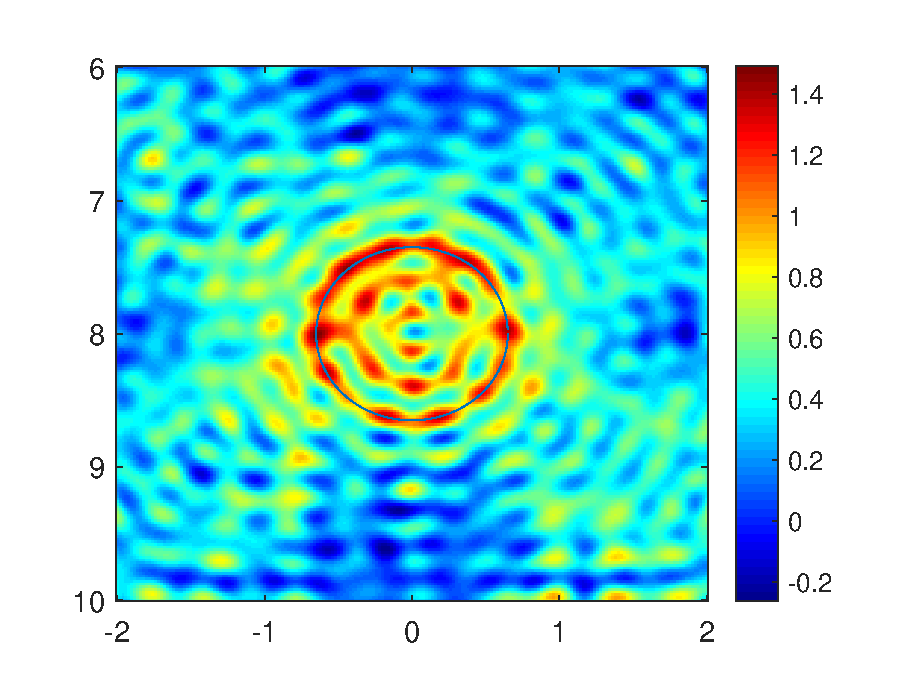
\includegraphics[width=0.23\textwidth]{./waveguide1/example3/In_transmission_circle_3.eps}
  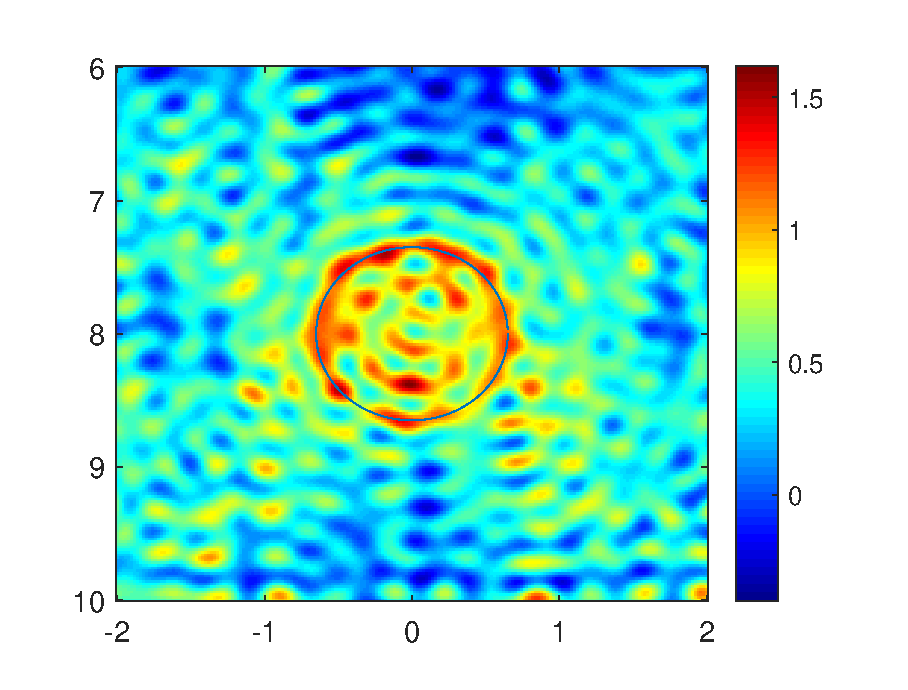
\includegraphics[width=0.23\textwidth]{./waveguide1/example3/In_transmission_circle_4.eps}
  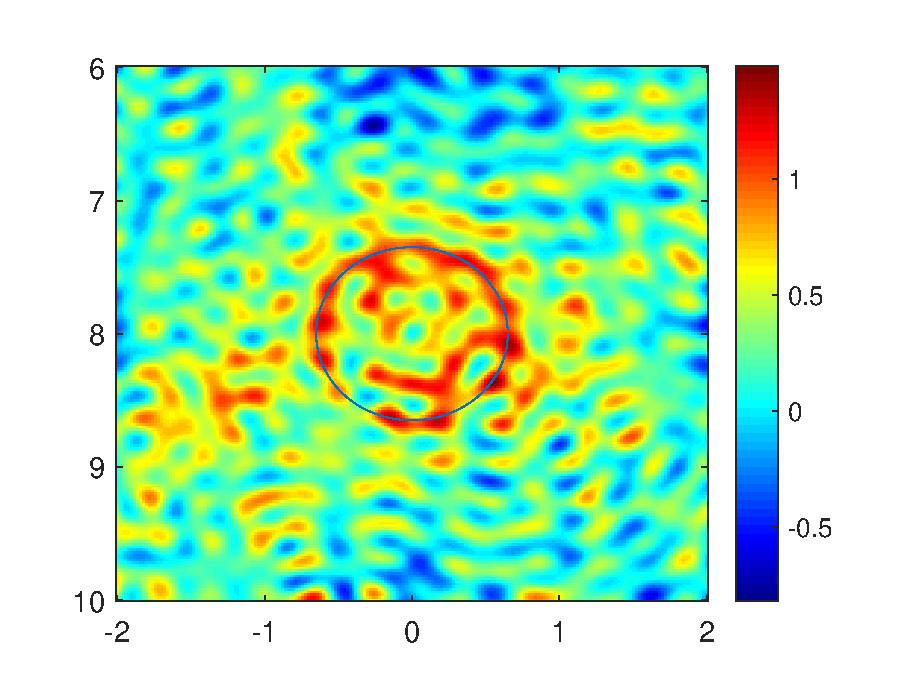
\includegraphics[width=0.23\textwidth]{./waveguide1/example3/In_transmission_circle_5.eps}
  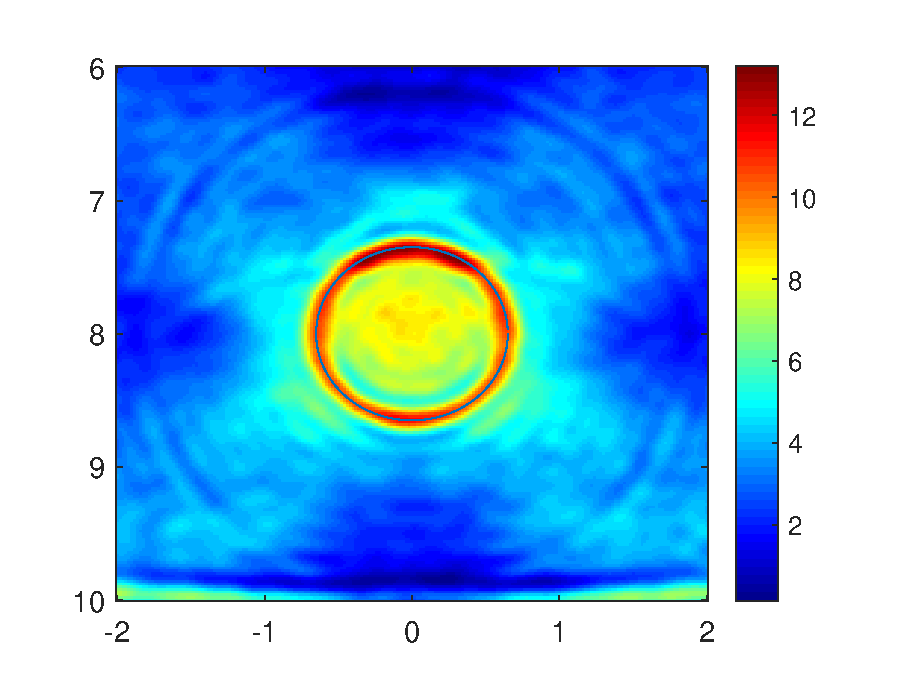
\includegraphics[width=0.23\textwidth]{./waveguide1/example3/In_transmission_circle_2_multi.eps}
  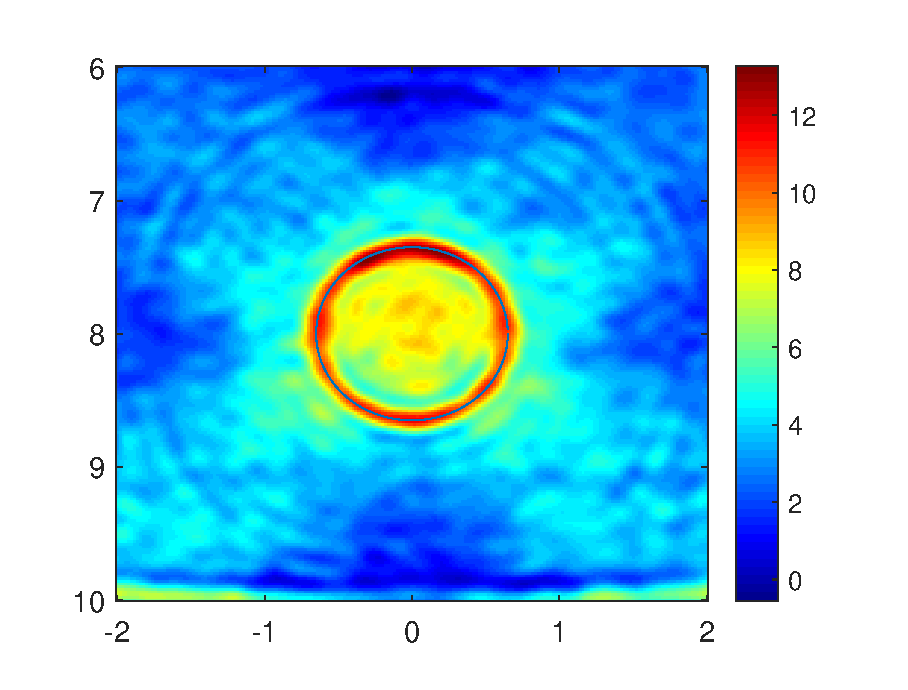
\includegraphics[width=0.23\textwidth]{./waveguide1/example3/In_transmission_circle_4_multi.eps}
  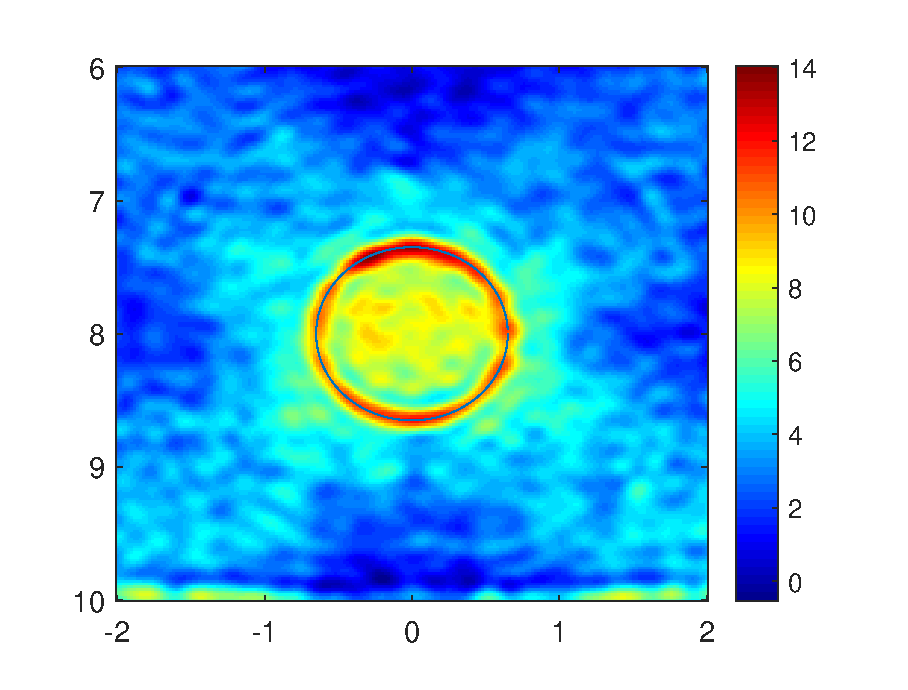
\includegraphics[width=0.23\textwidth]{./waveguide1/example3/In_transmission_circle_6_multi.eps}
  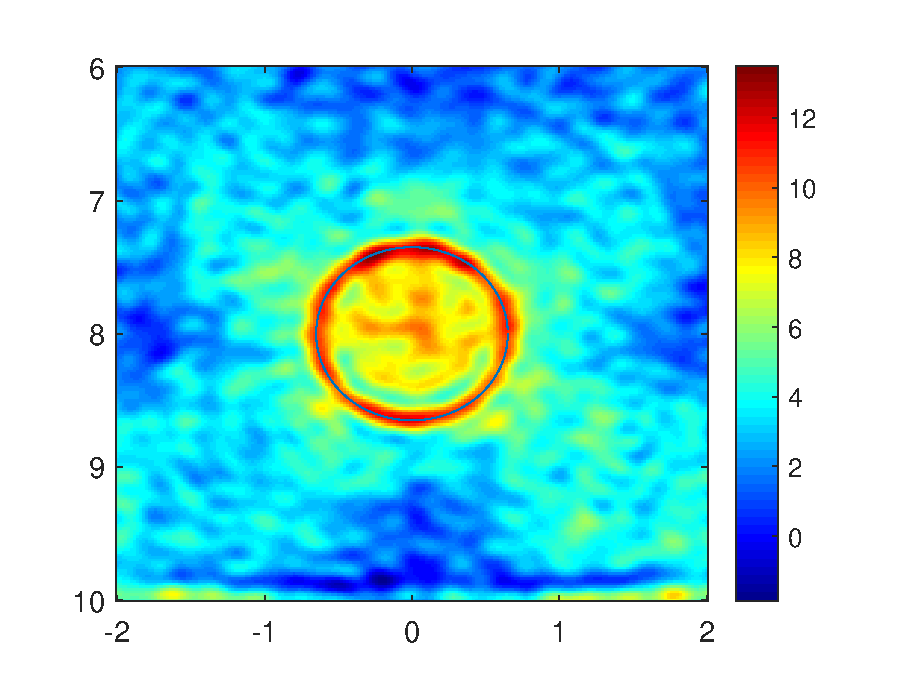
\includegraphics[width=0.23\textwidth]{./waveguide1/example3/In_transmission_circle_8_multi.eps}
  \caption{算例\ref{wg_ex3}:测试算法\ref{alg_wg}的抗噪音性能:目标障碍物为圆形的可穿透障碍物,噪音水平$\mu$从左到右按如下水平依次递增:$0.1,0.2,0.4,0.6$。其中第一行为单频测试结果,测试频率为:$k_1=4\pi,k_2=2\pi$;第二行为多频测试结果,测试频率为:$k_2=\frac{1}{2}k_1,k_1=2\pi+0.4n\pi,n=0,1\ldots,9$。}\label{fig_wg_ex3_2}
\end{figure}
\begin{remark}
	从本小节的数值算例可以看出,当目标障碍物$D$嵌入在Pekeris开波导第一层时,我们在上节所提出的算法\ref{alg_wg}能够对不同类型不同边界的障碍物进行有效成像,而且具有良好的抗噪性能。多频测试结果表明了算法定位目标的准确性以及多频能极大提高算法性能。除此之外,我们也发现,如果仅仅是探寻开波导第一层$L_1$内的障碍物,那么函数$G_{k_1}(x,z):=\Phi_{k_1}(x,z)-\Phi_{k_1}(x,z')$也是一种可选的反传播函数,其好处是反传播函数的计算速度极快以及计算精度较高。
\end{remark}
\subsection{障碍物$D\subset L_2$.}
在本小节中,我们考虑障碍物位于Pekeris开波导第二层$L_2$,即假设$D\subset L_2$。我们令$h=10,d=50$,且源点$x_s$ 和接收点$x_r$依旧 在$\Gamma_0^d$上均匀分布,其中$\Gamma_0^d=\{(x_1,x_2)\in\R^2;x_1\in(-d,d),x_2=0\}$。 采样区域为$\Omega=[-2,2]\times[10,14]$,且我们采用$201\times201$ 的均匀采样。为提高分辨率,取探测频率为$k_1=8\pi,k_2=4\pi$。 源点和接收点个数为$N_s=256,N_r=256$。
\begin{example}[不同边界类型]\label{wgout_ex1}
在本算例中,我们以圆形障碍物为例,验证算法\ref{alg_wg}对位于Pekeris 开波导第二层具有不同边界类型的障碍物的成像效果。例如声软障碍物,声硬障碍物,折射系数为$n(x)$ 的可穿透障碍物,阻尼系数为$\eta(x)$的阻抗边界障碍物。对于可穿透障碍物成像,我们假设折射系数$n(x)$ 为:
\begin{eqnarray*}
n(x)=\left\{
\begin{array}{lll}
  0.5&,&x\in D\\
  1&,&x\in\R_+^2\backslash\overline D
\end{array}
\right.
\end{eqnarray*}
对于阻抗边界障碍物,我们假设在上半边界$\eta(x)=1$,在下半边界$\eta(x)=2$。与之前一样,我们将使用相同的参数设定,来测试当反传播函数为$G_{k_1}(x,z)$时所对应的成像函数\eqref{Id_half}的成像效果。除此之外,我们将同样考虑反传播函数为$G_{k_2}(x,z):=\Phi_{k_2}(x,z)-\Phi_{k_2}(x,z')$时如下成像函数:
\begin{equation}\label{Id_half2}
I_d^{k_2}(z)=\Im\left\{\frac{|\Gamma_0^d|}{N_s}\frac{|\Gamma_0^d|}{N_r}\sum\limits_{s=1}^{N_s}\sum\limits_{r=1}^{N_r}\frac{\partial G_{k_2}(x_s,z)}{\partial x_2(x_s)}\frac{\partial G_{k_2}(x_r,z)}{\partial x_2(x_r)}\overline{u^s(x_r,x_s)}
\right\}.
\end{equation}
的成像效果。

测试结果如图\ref{fig_wgout_ex1}所示,从第一行可以看出:1. 即使没有提前知道障碍物的任何先验信息,如是否可穿透以及不可穿透障碍物的边界类型,算法\ref{alg_wg}的成像函数\eqref{Id_wg}都能够做到有效成像。2. 对于不可穿透障碍物,算法\ref{alg_wg}仅仅能确定障碍物的上边界信息;对于可穿透障碍物,算法\ref{alg_wg}能够确定障碍物上下两个边界的信息,但对于无法对侧边界进行有效成像。这与文献\cite{ch_ha}中的一般半空间情形是类似的,因为我们仅在$\Gamma_0^d$上接受数据,障碍物其他边界的散射信息并没有传播回来。

除此之外,从图\ref{fig_wgout_ex1}第二、三行可以看出,与点扩散函数的测试结果一致,若采用函数$G_{k_1}(x,z)$或$G_{k_2}(x,z)$来计算反传播过程和互相关,都不能确定障碍物的位置,大小和形状,所以直接将文献\cite{ch_ha,ch_cw}中的做法加以推广是行不通的。
\end{example}
\begin{figure}[h]
  \centering
  \includegraphics[width=0.23\textwidth]{./waveguide1/out_example1/out_circle_soft.eps}
  \includegraphics[width=0.23\textwidth]{./waveguide1/out_example1/out_circle_hard.eps}
  \includegraphics[width=0.23\textwidth]{./waveguide1/out_example1/out_circle_imp.eps}
  \includegraphics[width=0.23\textwidth]{./waveguide1/out_example1/out_circle_tran.eps}
  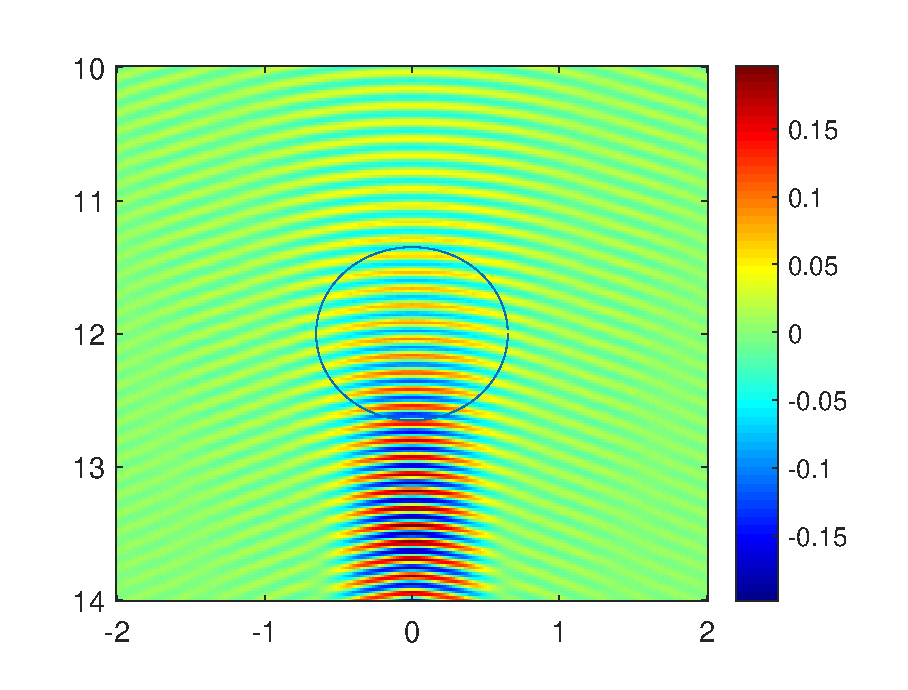
\includegraphics[width=0.23\textwidth]{./waveguide1/out_example1/out_circle_soft_half.eps}
  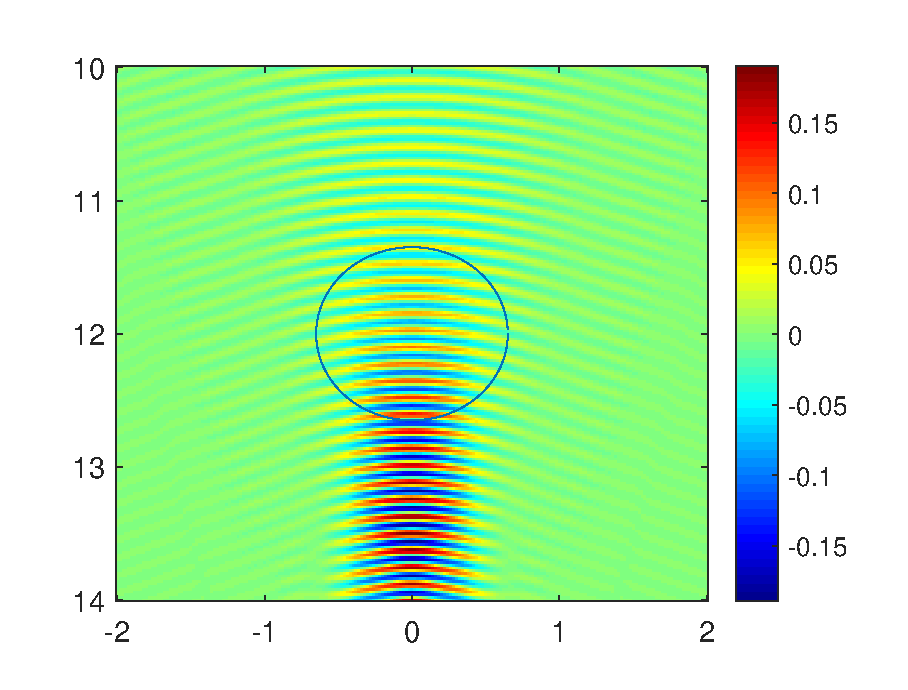
\includegraphics[width=0.23\textwidth]{./waveguide1/out_example1/out_circle_hard_half.eps}
  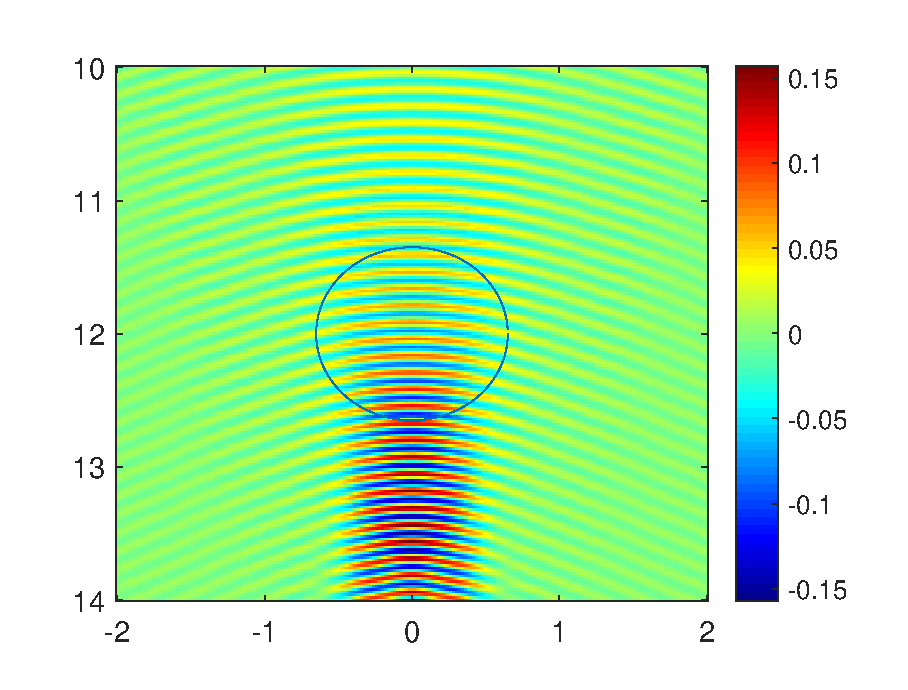
\includegraphics[width=0.23\textwidth]{./waveguide1/out_example1/out_circle_imp_half.eps}
  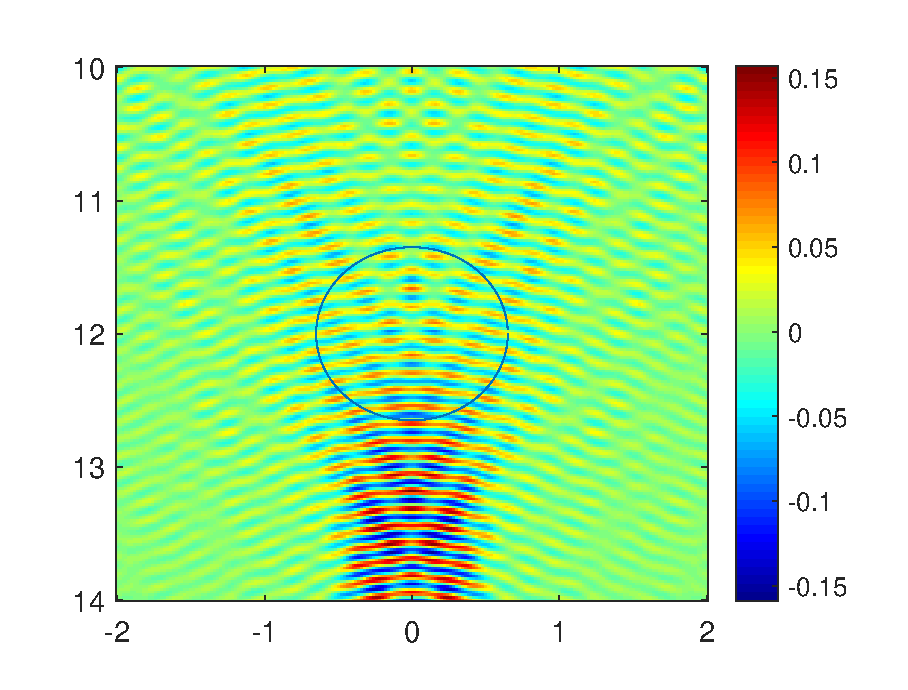
\includegraphics[width=0.23\textwidth]{./waveguide1/out_example1/out_circle_tran_half.eps}
  \includegraphics[width=0.23\textwidth]{./waveguide1/out_example1/out_circle_soft_half2.eps}
  \includegraphics[width=0.23\textwidth]{./waveguide1/out_example1/out_circle_hard_half2.eps}
  \includegraphics[width=0.23\textwidth]{./waveguide1/out_example1/out_circle_imp_half2.eps}
  \includegraphics[width=0.23\textwidth]{./waveguide1/out_example1/out_circle_tran_half2.eps}
  \caption{算例\ref{wgout_ex1}:测试位于Pekeris开波导第二层$L_2$的不同类型障碍物:前面三个从左到右依次为声软障碍物、声硬障碍物、阻尼系数为$\eta(x)$的阻抗边界障碍物,最后一个为折射系数为$n(x)$的可穿透障碍物,其中第一行为算法\ref{alg_wg}成像函数\ref{Id_wg}的成像效果,第二、三行分别为反传播函数是函数$G_{k_1}(x,z)$或$G_{k_2}(x,z)$时所对应成像函数\eqref{Id_half}或\eqref{Id_half2}的成像效果。}\label{fig_wgout_ex1}
\end{figure}
\begin{example}[不同形状]\label{wgout_ex2}
在本算例中,我们以声软障碍物和可穿透障碍物为例测试位于Pekeris 开波导第二层具有不同形状的障碍物,例如4叶风扇形状,矩形形状,花生形状和椭圆形状,算法
\ref{alg_wg}的成像效果。

测试结果如图\ref{fig_wgout_ex2}所示,结果表明:对位于Pekeris开波导第二层$L_2$的不同形状的障碍物$D$,算法\ref{alg_wg}中的成像函数\ref{Id_wg}都能够做到有效成像。其成像效果类似于文献\cite{ch_ha}中一般半空间情形:1. 由于在$\Gamma_0^d$上接收到的散射数据不包含不可穿透障碍物下边界信息,故而仅能对声软障碍物上边界进行成像;2. 对于可穿透障碍物,算法\ref{alg_wg}不仅可以确定障碍物的上半边界,而且对障碍物的下半边界也可以进行成像,这也是符合情理的。
\end{example}
\begin{figure}[h]
  \centering
  \includegraphics[width=0.23\textwidth]{./waveguide1/out_example2/Out_soft_pleaf1.eps}
  \includegraphics[width=0.23\textwidth]{./waveguide1/out_example2/Out_soft_square1.eps}
  \includegraphics[width=0.23\textwidth]{./waveguide1/out_example2/Out_soft_peanut.eps}
  \includegraphics[width=0.23\textwidth]{./waveguide1/out_example2/Out_soft_circle1.eps}
  \includegraphics[width=0.23\textwidth]{./waveguide1/out_example2/Out_tran_pleaf1.eps}
  \includegraphics[width=0.23\textwidth]{./waveguide1/out_example2/Out_tran_square1.eps}
  \includegraphics[width=0.23\textwidth]{./waveguide1/out_example2/Out_tran_peanut.eps}
  \includegraphics[width=0.23\textwidth]{./waveguide1/out_example2/Out_tran_circle1.eps}
  \caption{算例\ref{wg_ex2}:测试对于Pekeris开波导第二层$L_2$的不同类型不同形状的障碍物:从左到右依次为4叶风扇、矩形、花生以及椭圆形状,其中第一行为声软障碍物,第二行为可穿透障碍物。}
  \label{fig_wgout_ex2}
\end{figure}
\begin{example}[抗噪性及多频测试]\label{wgout_ex3}
在本算例中,我们测试在$\Gamma_0^d$上接收到的散射数据$u^s(x_r,x_s)$带有高斯噪音时,算法\ref{alg_wg} 对位于Pekeris开波导第二层障碍物成像的抗噪性能。设$u^s_{noise}(x_r,x_s)$ 为如下带有高斯噪音的散射数据:
$$ u^s_{noise}(x_r,x_s)=u^s(x_r,x_s)+v_{noise},$$
其中$v_{noise}$为满足如下分布的高斯噪音:
$$v_{noise}=\mu \max{|u^s|}\epsilon,\ \ \epsilon\sim N(0,1).$$

测试结果如图\ref{fig_wgout_ex3}所示:障碍物为4-叶风扇形状的声软障碍物,噪音水平$\mu$从左到右按如下数值依次递增:$0.1,0.2,0.4,0.6$,第一行为单频测试结果,测试频率为$k_1=8\pi,k_2=4\pi$,第二行为多频测试结果,测试频率为$k_2=\frac{1}{2}k_1,k_1=4\pi+0.4n\pi,n=0,1,\ldots,6$。结果表明算法:\ref{alg_wg}中的成像函数\eqref{Id_wg}具有十分良好的抗噪性能;此外多频叠加能够很好得改善成像效果,提升算法抗噪性能。
\end{example}
\begin{figure}[h]
  \centering
  \includegraphics[width=0.23\textwidth]{./waveguide1/out_example3/Out_soft_pleaf1_2.eps}
  \includegraphics[width=0.23\textwidth]{./waveguide1/out_example3/Out_soft_pleaf1_4.eps}
  \includegraphics[width=0.23\textwidth]{./waveguide1/out_example3/Out_soft_pleaf1_6.eps}
  \includegraphics[width=0.23\textwidth]{./waveguide1/out_example3/Out_soft_pleaf1_8.eps}
  \includegraphics[width=0.23\textwidth]{./waveguide1/out_example3/Out_soft_pleaf1_2_multi.eps}
  \includegraphics[width=0.23\textwidth]{./waveguide1/out_example3/Out_soft_pleaf1_4_multi.eps}
  \includegraphics[width=0.23\textwidth]{./waveguide1/out_example3/Out_soft_pleaf1_6_multi.eps}
  \includegraphics[width=0.23\textwidth]{./waveguide1/out_example3/Out_soft_pleaf1_8_multi.eps}
  \caption{算例\ref{wgout_ex3}:测试算法\ref{alg_wg}的抗噪音性能:目标障碍物为位于开波导第二层$L_2$的4-叶风扇形状的声软障碍物,噪音水平$\mu$从左到右按如下数值依次递增:$0.1,0.2,0.4,0.6$。其中第一行为单频测试结果,测试频率为:$k_1=8\pi,k_2=4\pi$;第二行为多频测试结果,测试频率为:$k_2=\frac{1}{2}k_1,k_1=4\pi+0.4n\pi,n=0,1,\ldots,6$。}\label{fig_wgout_ex3}
\end{figure}
%\begin{example}
%在本算例中,我们测试在$L_2$层中具有两个障碍物时,算法的成像效果。
%
%\end{example}
%\begin{figure}[h]
%  \centering
%  \includegraphics[width=0.23\textwidth]{./waveguide1/out_example4/Out_twosoft_single_2.eps}
%  \includegraphics[width=0.23\textwidth]{./waveguide1/out_example4/Out_twosoft_single_4.eps}
%  \includegraphics[width=0.23\textwidth]{./waveguide1/out_example4/Out_twosoft_single_6.eps}
%  \includegraphics[width=0.23\textwidth]{./waveguide1/out_example4/Out_twosoft_single_8.eps}
%  \includegraphics[width=0.23\textwidth]{./waveguide1/out_example4/Out_twosoft_multi_2.eps}
%  \includegraphics[width=0.23\textwidth]{./waveguide1/out_example4/Out_twosoft_multi_4.eps}
%  \includegraphics[width=0.23\textwidth]{./waveguide1/out_example4/Out_twosoft_multi_6.eps}
%  \includegraphics[width=0.23\textwidth]{./waveguide1/out_example4/Out_twosoft_multi_8.eps}
%    \caption{算例\ref{wgout_ex3}:障碍物位于$L_2$层,单频带噪音数据测试,噪音水平$\mu$从左到右依次为$0.1,0.2,0.4,0.6$}\label{fig_wgout_ex4}
%\end{figure}
\begin{remark}
	从本小节的数值测试可以看出,当目标障碍物$D$嵌入在Pekeris开波导第二层时,我们在上节所提出的算法\ref{alg_wg}同样能够对不同类型不同边界的障碍物进行有效成像,而且抗噪性能和多频测试也都达到了预期效果。此外,测试表明:当$D\subset L_2$时,采用$G_{k_1}(x,z):=\Phi_{k_1}(x,z)-\Phi_{k_1}(x,z')$
	或$G_{k_2}(x,z):=\Phi_{k_2}(x,z)-\Phi_{k_2}(x,z')$来计算反传播场和互相关不再合适。通过对比,我们发现了算法\ref{alg_wg}具有良好的可扩展性,可以考虑将算法推广到半空间三层开波导,甚至是任意层的开波导模型,这也是我们下一步的研究方向之一。
\end{remark}

\section{算法分析与思考}
我们通过对点扩散函数的测试提出了适用于Pekeris开波导障碍物成像问题的逆时偏移算法\ref{alg_wg},并且通过大量的数值算例验证了算法的可行性。对于算法\ref{alg_wg}的分辨率分析同样需要从点扩散函数开始,在对有限孔穴点扩散函数进行分析时发现一个很有意思的问题,该问题对孔穴半径的选取起到十分重要的影响。

设孔穴$d>0$,以及$\Gamma_0^d:=\{(x_1,x_2)\in\R^2_+\}$,则对应于算法\ref{alg_wg}的有限孔穴点扩散函数为:
\begin{equation}
 J_d(z,y)=\int_{\Gamma_0^d}\frac{\partial G(x_r,z)}{\partial x_2(x_r)}\overline{N(x_r,y)}ds(x_r)
\end{equation}
其中$G(x,z),N(x,y)$分别为Pekeris开波导Dirichlet和Neumann格林函数。
我们首先要考虑如下问题:
\begin{question}\label{pro_convergence}
当孔穴半径$d\rightarrow+\infty$时,极限$\lim\limits_{d\rightarrow+\infty}J_d(z,y)$是否点点收敛?
\end{question}
根据定理\ref{Dirichlet_Mode} 和定理\ref{Neumann_Mode}可知,函数$G(x,z)$和$N(x,y)$都会产生波导模式:
\begin{eqnarray*}
  G(x,z)=G_g(x,z)+G_{rad}(x,z),\ \
  N(x,y)=N_g(x,y)+N_{rad}(x,y)
\end{eqnarray*}
其中$G_g(x,z)=\sum\limits_{p=1}^MG_p(x,z)$ 和$N_g(x,y)=\sum\limits_{q=1}^{\hat M}N_q(x,y)$,分别为格林函数$G(x,z)$和$N(x,y)$的波导项,$G_{rad}(x,z)$和$N_{rad}(x,y)$分别为相应衰减项。则此时有限孔穴点扩散函数$J_d(z,y)$可以分成四个部分:
\begin{equation}
  J_d(z,y)=J_d^1(z,y)+J_d^2(z,y)+J_d^3(z,y)+J_d^4(z,y)
\end{equation}
其中$J_d^i(z,y),i=1,2,3,4$为
\begin{eqnarray}\label{psf_wg_4p}
 \left\{
 \begin{array}{lll}
  J_d^1(z,y)&=&\int_{\Gamma_0^d}\frac{\partial G_g(x_r,z)}{\partial x_2(x_r)}\overline{N_g(x_r,y)}ds(x_r)\\
  & &\\
  J_d^2(z,y)&=&\int_{\Gamma_0^d}\frac{\partial G_{rad}(x_r,z)}{\partial x_2(x_r)}\overline{N_{rad}(x_r,y)}ds(x_r)\\
  & &\\
  J_d^3(z,y)&=&\int_{\Gamma_0^d}\frac{\partial G_g(x_r,z)}{\partial x_2(x_r)}\overline{N_{rad}(x_r,y)}ds(x_r)\\
  & &\\
  J_d^4(z,y)&=&\int_{\Gamma_0^d}\frac{\partial G_{rad}(x_r,z)}{\partial x_2(x_r)}\overline{N_g(x_r,y)}ds(x_r)
 \end{array}
 \right.
\end{eqnarray}

这里的$J_d^1(z,y)$表示$G(x,y)$的波导项反传$N(x,y)$的波导项,$J_d^2(z,y)$为衰减项反传衰减项,而$J_d^i(z,y),i=3,4$表示交叉反传项。从第三节的数值测试可知:当$z=y$时,$-\Im J_d(z,y)$取得峰值,然后$|z-y|$变大时其逐渐衰减。对于一般半空间模型,文献\cite{ch_ha}基于点扩散函数的这个性质,提出了半空间逆时偏移算法,这同时也是逆时偏移算法分辨率分析的难点和关键点。

与文献\cite{ch_ha}中一般半空间情形不同的是,开波导模型逆时偏移算法的点扩散函数包含如上四个不同的部分,首先我们要通过测试来观察哪些成分在点扩散函数$J_d^{z,y}$中起到主要的作用。令$h=10,d=50$,然后设第一个源点为在$L_1$层内的$y_1=(0,5)$,取采样区域为$\Omega_1=[-2,2]\times[3,7]$;第二个源点为在$L_2$层内的$y_2=(0,15)$,去采样区域为$\Omega_2=[-2,2]\times[13,17]$。
\begin{figure}[htbp]
	\centering
	\includegraphics[width=0.23\textwidth]{./waveguide1/psf_part/psf_wg_in_1}
	\includegraphics[width=0.23\textwidth]{./waveguide1/psf_part/psf_wg_in_2}
	\includegraphics[width=0.23\textwidth]{./waveguide1/psf_part/psf_wg_in_3}
	\includegraphics[width=0.23\textwidth]{./waveguide1/psf_part/psf_wg_in_4}
	\caption{点扩散函数测试:$-\Im f(z,y)$,其中源点$y_1=(0,5)$在开波导第一层$L_1$内,从左到右函数$f(z,y)$依次为波导项反传波导项$J_d^1(z,y)$,衰减项反传衰减项$J_d^2(z,y)$,以及交叉反传项$J_d^3(z,y)$和$J_d^4(z,y)$。其中采样区域为$\Omega_1=[-2,2]\times[3,7]$,以及$k_2=\frac{1}{2}k_1,k_1=[2\pi,4\pi,6\pi]$。}\label{psf_wg_part_in}
\end{figure}
\begin{figure}[htbp]
	\centering
	\includegraphics[width=0.23\textwidth]{./waveguide1/psf_part/psf_wg_out_1}
	\includegraphics[width=0.23\textwidth]{./waveguide1/psf_part/psf_wg_out_2}
	\includegraphics[width=0.23\textwidth]{./waveguide1/psf_part/psf_wg_out_3}
	\includegraphics[width=0.23\textwidth]{./waveguide1/psf_part/psf_wg_out_4}
	\caption{点扩散函数测试:$-\Im f(z,y)$,其中源点$y_2=(0,15)$在开波导第二层$L_2$内,从左到右函数$f(z,y)$依次为波导项反传波导项$J_d^1(z,y)$,衰减项反传衰减项$J_d^2(z,y)$,以及交叉反传项$J_d^3(z,y)$和$J_d^4(z,y)$。其中采样区域为$\Omega_1=[-2,2]\times[13,17]$,以及$k_2=\frac{1}{2}k_1,k_1=[4\pi,6\pi,8\pi]$。}\label{psf_wg_part_out}
\end{figure}
测试结果如图\ref{psf_wg_part_in}和图\ref{psf_wg_part_out}所示。结果表明:
\begin{itemize}
	\item 当源点$y\in L_1$时,点扩散函数$J_d(z,y)$中起关键作用的为波导项反传波导项$J^1_d(z,y)$和衰减项反传衰减项$J^2_d(z,y)$,而交叉反传项不起作用;
	\item 当源点$y\in L_2$时,点扩散函数$J_d(z,y)$中起关键作用的为衰减项反传衰减项,而其他三项不起作用。
\end{itemize}

在对其做进一步的分析时,我们发现一个非常致命但又有意思的问题:

\begin{question}\label{pro_fatal}
 当$d\rightarrow+\infty$时,波导项反传波导项$J_d^1(z,y)$并不收敛,但是当源点$y\in L_1$时,两个格林函数的波导项按照$J_d^1(z,y)$互相作用会具有如图\ref{psf_wg_part_in}第一项所示的良好性质:当$z=y$时,$-Im J_d^1(z,y)$取得峰值;当$|z-y|$变大,$-\Im J_d^1(z,y)$逐渐衰减。
\end{question}

事实上,由定理\ref{Dirichlet_Mode}和定理\ref{Neumann_Mode}可知,波导模式$G_g(x,z)=\sum\limits_{p=1}^MG_p(x,z)$ 和$N_g(x,y)=\sum\limits_{q=1}^{\hat M}N_q(x,y)$ 的各个分量具体表达式如下
\begin{eqnarray*}
 \left\{
 \begin{array}{lll}
    G_p(x,z)&=&\frac{\mu_{2p}}{\xi_p(1-\i\mu_{2p}h)}g(x_2,\xi_p)g(z_2,\xi_p)e^{\i|x_1-z_1|\xi_p}\\
    & &\\
    N_p(x,y)&=&\frac{\hat\mu_{2q}}{\hat\xi_q(1-\i\hat\mu_{2q}h)}\hat g(x_2,\hat\xi_q)\hat g(y_2,\hat\xi_m)e^{\i|x_1-y_1|\hat\xi_m}\\
 \end{array}
 \right.
\end{eqnarray*}
 其中函数$g(x_2,\xi_p)$ 和$\hat g(x_2,\hat\xi_q)$分别为
 \begin{eqnarray*}
 g(x_2,\xi_p):=\left\{
 \begin{array}{lll}
   \sin(\mu_{1p}x_2),& &x_2\in(0,h)\\
   & &\\
   \sin(\mu_{1p}h)e^{\i\mu_{2p}(x_2-h)},& &x_2\in(h,+\infty)
 \end{array}
 \right.
 \end{eqnarray*}
 和
\begin{eqnarray*}
\hat g(x_2,\hat\xi_q):=\left\{
 \begin{array}{lll}
   \cos(\hat\mu_{1q}x_2),& &x_2\in(0,h)\\
   & &\\
   \cos(\hat\mu_{1q}h)e^{\i\hat\mu_{2q}(x_2-h)},& &x_2\in(h,+\infty)
 \end{array}
 \right.
\end{eqnarray*}
此外,$\xi_p,p=1,2,\ldots,M;\hat\xi_q,q=1,2,\ldots,\hat M$ 为如下两个函数
\begin{eqnarray*}
N_h(\xi):=\frac{\mu_1+\mu_2}{\mu_1-\mu_2}+e^{2\i\mu_1h},\ \
\hat N_h(\xi):=\frac{\mu_1+\mu_2}{\mu_1-\mu_2}-e^{2\i\mu_1h}
\end{eqnarray*}
在区间$(k_2,k_1)$上的根,以及$\mu_{1p},\mu_{2p},\hat\mu_{1q},\hat\mu_{2q}$ 分别为
\begin{eqnarray*}
\begin{array}{lllllll}
\mu_{1p}=\sqrt{k_1^2-\xi_p^2}&,&\mu_{2p}=\sqrt{k_2^2-\xi_p^2}&,&\hat\mu_{1q}=\sqrt{k_1^2-\hat\xi_q^2}&,&
\hat\mu_{2q}=\sqrt{k_2^2-\hat\xi_q^2},
\end{array}
\end{eqnarray*}
直接代入式\ref{psf_wg_4p}的第一项,即可得到$J_d^1(z,y)$ 的具体表达式,具体如下述引理所示:
\begin{lemma}\label{psf_wg_Jd1}
\begin{equation}
  J_d^1(z,y)=\sum\limits_{p=1}^M\sum\limits_{q=1}^{\hat M}f_{pq}(z_2,y_2)I^{pq}_d(z_1,y_1)
\end{equation}
其中
\begin{equation}
I^{pq}_d(z_1,y_1) =\int_{-d}^{d}e^{\i|x_1-z_1|\xi_p-\i|x_1-y_1|\hat\xi_q}dx_1
\end{equation}
此外,$f_{pq}(z_2,y_2),p=1,2\ldots,M;q=1,2,\ldots,\hat M$ 是关于$z_2$和$y_2$的函数。
\end{lemma}
\begin{remark}\label{Idm1m2}
直接计算可得$I_d^{pq}(z_1,y_1)$的具体表达式:当$z_1,y_1\in(-d,d)$时,
\begin{equation}
  I_d^{pq}(z_1,y_1)=\psi^{pq}_1(d,z_1,y_1)+\psi^{pq}_2(z_1,y_1)
\end{equation}
其中
\begin{eqnarray*}
\left\{
\begin{array}{lll}
  \psi^{pq}_1(d,z_1,y_1)&=&\frac{e^{\i d(\xi_{p}-\hat\xi_{q})}}{\i(\xi_{p}-\hat\xi_{q})}\left(e^{\i z_1\xi_{p}-\i y_1\hat\xi_{q}}+e^{\i y_1\hat\xi_{q}-\i z_1\xi_{p}}\right)\\
  & &\\
  \psi^{pq}_2(z_1,y_1)&=&\frac{e^{\i|z_1-y_1|\xi_{p}}-e^{-\i|z_1-y_1|\hat\xi_{q}}}{\i(\xi_{p}+\hat\xi_{q})}
-\frac{e^{\i|z_1-y_1|\xi_{p}}+e^{-\i|z_1-y_1|\hat\xi_{q}}}{\i(\xi_{p}-\hat\xi_{q})}
\end{array}
\right.
\end{eqnarray*}
\end{remark}

由引理\ref{psf_wg_Jd1}和注\ref{Idm1m2}可知,有限孔穴点扩散函数的第一项$J_d^1(z,y)$为:
\begin{eqnarray}
J_d^1(z,y)=\sum\limits_{p=1}^M\sum\limits_{q=1}^{\hat M}f_{pq}(z_2,y_2)\psi^{pq}_1(d,z_1,y_1)+
\sum\limits_{p=1}^M\sum\limits_{q=1}^{\hat M}f_{pq}(z_2,y_2)\psi^{pq}_2(z_1,y_1)\qquad
\end{eqnarray}
直接观察可知:上式中第二项与孔穴半径$d$无关,仅仅第一项中的因子
$$\psi^{pq}_1(d,z_1,y_1)$$
与孔穴半径$d$相关。但是极限
\begin{equation}
 \lim\limits_{d\rightarrow+\infty}e^{\i d(\xi_{p}-\hat\xi_{q})}
\end{equation}
并不收敛,这导致了极限
\begin{equation}
\lim\limits_{d\rightarrow+\infty}J_d^1(z,y)
\end{equation}
的收敛性无从保证。如何确定选取合适孔穴半径$d$ 的规则就成为一个比较棘手的问题。所以对于问题\ref{pro_convergence},我们并没有得到满意的答案。从之前的数值测试可以看出算法\ref{alg_wg}成像的有效性,然而通过现有的手段已经无法建立其合适的分辨率分析以及确定选取孔穴半径的法则,其分析需要更高级的数学工具,这也是我们今后工作的研究方向之一。

\begin{remark}
	值得一提的是,对于在本文第一章所介绍的平板声波闭波导模型,同样存在类似于问题\ref{pro_fatal}的现象。文献\cite{ch_cw}针对平板声波闭波导障碍物成像问题,提出了一种采用半空间格林函数$G_k(x,z):=\Phi_k(x,z)-\Phi_{k}(x,z)$做为反传播函数的闭波导逆时偏移算法,并且建立了严格的分辨率分析和进行了大量的数值测试。事实上,比较自然的反传播函数是Dirichlet零边界的格林函数,那么此时就会产生类似于问题\ref{pro_fatal}的现象。闭波导模型相对于开波导略微容易,故而在可以尝试先从闭波导模型入手。由于本文主要研究开波导障碍物成像问题,我们将关于闭波导类似的讨论放在本文附录,这也是我们感兴趣的一个问题。
\end{remark}
\section{本章小结}
本章通过对点扩散函数的分析和测试,提出了一种开波导逆时偏移算法。该算法继承了一般半空间逆时偏移算法的优点,在不需要障碍物的先验信息的情况下,能够对位于Pekeris 开波导不同层的不同障碍物进行成像。然后我们发现了开波导逆时偏移算法的有限孔穴点扩散函数存在收敛性问题\ref{pro_convergence}。从数值测试结果来看,即便问题\ref{pro_convergence} 的存在,所选取的反传播函数,也就是Pekeris开波导Dirichlet 格林函数依然能够处理波导模型本身的多次反射波。在下一章,我们将继续对开波导障碍物成像问题进行讨论,并且探索出了一种新的逆时偏移算法。


%\section{算法分析与解释}
%由于当障碍物位于开波导不同区域时成像效果并不一样,故而下面我们分别对其成效效果进行分析,并解释说明成像效果不同的原因。
%\subsection{障碍物$D\subset L_1$}
%为说明有点孔径点扩散函数的收敛性,我们先分析反传播函数$G_h(x,z)$在$x_1$方向上的衰减性。
%\begin{lemma}[$G_h(x,z)$ 的衰减性分析]
%假设$x\in\Gamma_0$, $\kappa:=\frac{k_2}{k_1}$, $k_1|x-y|>1$ 以及
%\begin{equation}
%  \frac{|x_1-y_1|}{|x-y|}>\frac{1+\kappa}{2},\ \ \frac{y_2}{|x-y|}<\frac{\kappa}{2}
%\end{equation}
%则我们有\\
%$(1)$ 当$y\in L_1$时,
%\begin{equation}
%  \left|\frac{\partial G_h(x,y)}{\partial x_2}\right|\leq Ck_1\left[
%  \frac{y_2}{|x-y|}\frac{1}{(k_1|x-y|)^{\frac{1}{2}}}+\frac{|x_1-y_1|}{|x-y|}\frac{1}{(k_1|x-y|)^{\frac{3}{2}}}
%  \right]
%\end{equation}
%其中常数$C$与$k_1,k_2,h,x,y$ 无关。\\
%$(2)$ 当$y\in L_2$ 时,????
%\end{lemma}
%由上述引理可知我们所定义的点扩散函数是绝对收敛的,然后我们的主要目标是完成下述两个定理。
%\begin{theorem}[提取$J(z,y)$ 的主项]\label{main_twolayer}
%设$\Omega$为采样区域,其满足假设\eqref{ass_sample},若定义函数$f_h(\xi),\xi\in(-k_1,k_1)$ 为
%\begin{eqnarray*}
%f_h(\xi)=\left\{
%\begin{array}{lll}
%\frac{(\mu_1-\mu_2)^2}{(\mu_1+\mu_2)^2-(k_1^2-k_2^2)e^{-2\i\mu_1h}},&if&\xi\in(-k_2,k_2)\\
%& &\\
%1,&if&\xi\in(-k_1,-k_2)\cup(k_2,k_1)
%\end{array}
%\right.
%\end{eqnarray*}
%以及函数$g_h(\xi),\xi\in(-k_2,k_2)$ 为
%\begin{eqnarray*}
% g_h(\xi)=\frac{4\mu_1\mu_2}{(\mu_1+\mu_2)^2-(\mu_1^2-\mu_2^2)e^{-2\i\mu_1h}}
%\end{eqnarray*}
%则点扩散函数$J(z,y)$有如下表示,\\
%$(1)$ 当$y\in L_1$时
%\begin{eqnarray*}
%  J(z,y)=\left\{
%  \begin{array}{lll}
%    F_1(z,y)+R_1(z,y)&,&z\in L_1\\
%    Q_1(z,y)&,&z\in  L_2\\
%  \end{array}
%\right.
%\end{eqnarray*}
%$(2)$ 当$y\in  L_2$时
%\begin{eqnarray*}
%  J(z,y)=\left\{
%  \begin{array}{lll}
%    Q_2(z,y)&,&z\in L_1\\
%    F_2(z,y)+R_2(z,y)&,&z\in  L_2\\
%  \end{array}
%\right.
%\end{eqnarray*}
%其中 $F_1(z,y),F_2(z,y)$的表达式如下式所示
%\begin{eqnarray*}
% F_1(z,y)&=&-\frac{\i}{4\pi}\int_{-k_1}^{k_1}\frac{1}{\mu_1}e^{\i\mu_1(z_2-y_2)+\i\xi(y_1-z_1)}d\xi
% -\frac{\i}{4\pi}\int_{-k_1}^{k_1}\frac{f_h(\xi)}{\mu_1}e^{\i\mu_1(y_2-z_2)+\i\xi(y_1-z_1)}d\xi\\
% F_2(z,y)&=&-\frac{\i}{4\pi}\int_{-k_2}^{k_2}\frac{g_h(\xi)}{\mu_2}
% e^{\i\mu_2(z_2-y_2)+\i\xi(y_1-z_1)}d\xi
%\end{eqnarray*}
%而$R_1(z,y),R_2(z,y),Q_1(z,y),Q_2(z,y)$ 为余项,且当$z,y$ 均位于采样区域$\Omega$时,我们有如下估计
%\begin{eqnarray*}
% |R_1(z,y)|\leq C\frac{k_1^2}{k_2^2}\frac{1}{\sqrt{k_1h}},\  \ z\in\Omega\cap L_1;\ \
% |R_2(z,y)|\leq C\frac{k_1^2}{k_2^2}\frac{1}{\sqrt{k_1h}},\  \ z\in\Omega\cap L_2\quad\quad\quad\\
% |Q_1(z,y)|\leq C\frac{k_1^2}{k_2^2}\frac{1}{\sqrt{k_1h}},\  \ z\in\Omega\cap L_1;\ \
% |Q_2(z,y)|\leq C\frac{k_1^2}{k_2^2}\frac{1}{\sqrt{k_1h}},\  \ z\in\Omega\cap L_2\quad\quad\quad
%\end{eqnarray*}
%\end{theorem}
%\debproof
%定义$J_{\epsilon}(z,y)$ 如下,
%\begin{eqnarray*}
% J_{\epsilon}(z,y)=\int_{\Gamma_0}\frac{\partial G(x,z)}{\partial x_2}\overline{N_{\epsilon}(x,y)}ds(x)
%\end{eqnarray*}
%其中$N_{\epsilon}(x,y)$ 是波数为$k(x)+\i\epsilon$的开波导Neumann格林函数,
%\begin{eqnarray*}
%\left\{
%\begin{array}{lll}
%  \Delta_x N_{\epsilon}(x,y)+[k(x)+\i\epsilon]^2N_{\epsilon}(x,y)=-\delta_y(x),&in&  \R_+^2;\\
%  & &\\
%  \frac{\partial N_{\epsilon}(x,y)}{\partial x_2}=0,& on&\Gamma_0.
%\end{array}
%\right.
%\end{eqnarray*}
%定义关于$x_1$分量的Fourier变换如下
%\begin{equation}
%    \hat{f}(\xi,x_2;y_1,y_2)=\int_{-\infty}^{\infty}f(x,y)e^{-\i x_1\xi}dx_1
%\end{equation}
%则直接计算可得
%\begin{eqnarray*}
%\frac{\partial \hat{G} (\xi,x_2;z_1,z_2)}{\partial x_2}\Bigg|_{x_2=0}=\left\{
%\begin{array}{lll}
%   \frac{1}{2}e^{\i\mu_1z_2-\i\xi z_1}+\frac{1}{2}\frac{\mu_1-\mu_2}{\mu_1+\mu_2}e^{\i\mu_1(2h-z_2)-\i\xi z_1}&,&z\in L_1\\
%   & &\\
%   \frac{\mu_1}{\mu_1+\mu_2}e^{\i\mu_2(z_2-h)+\i\mu_1h-\i\xi z_1}&,&z\in L_2
%\end{array}
%\right.
%\end{eqnarray*}
%以及
%\begin{eqnarray*}
%\hat N_{\epsilon}(\xi,0;y_1,y_2)=\left\{
%\begin{array}{lll}
%\frac{\i}{\mu_{1\epsilon}}e^{\i\mu_{1\epsilon}y_2-\i\xi y_1}+
%   \frac{\i}{\mu_{1\epsilon}}\frac{1}{N_0(\mu_{1\epsilon})}\left[e^{\i\mu_{1\epsilon}(2h+y_2)-\i\xi y_1}+
%   e^{\i\mu_{1\epsilon}(2h-y_2)-\i\xi y_1}\right]&,&y\in L_1\\
% & &\\
%  \frac{2\i}{\mu_{1\epsilon}-\mu_{2\epsilon}}\frac{1}{N_0(\mu_{1\epsilon})}
% e^{\i\mu_{2\epsilon}(y_2-h)+\i\mu_{1\epsilon}h-\i\xi y_1}&,&y\in L_2
%\end{array}
%\right.
%\end{eqnarray*}
%下面我们以$z,y\in L_2$ 为例来完成该定理的证明。当$z,y\in L_2$时,
%\finproof
%在下述定理中,我们对$F_1(z,y)$和$F_2(z,y)$进行估计。
%\begin{theorem}[$J(z,y)$ 的主项估计]
%令$F_1(z,y)$和$F_2(z,y)$如定理\ref{main_twolayer}中所示,则他们有如下性质,\\
%$(1)$ 当$z=y$时,$F_1(z,y)=-\i/4+?$ $F_2(z,y)=?$\\
%$(2)$ 当$|z-y|>0$时,
%\begin{eqnarray*}
% |F_1(z,y)|&\leq &C\left[(k_1|z-y|)^{-1/2}+(k_1|z-y|^{-1})\right],\\
% |F_2(z,y)|&\leq &C\left[(k_2|z-y|)^{-1/2}+(k_2|z-y|^{-1})\right].
%\end{eqnarray*}
%其中常数$C$与$k_1,k_2,|z-y|$ 无关,但与$h$有关。
%\end{theorem}
%\debproof
%令$\xi=k_1\sin\theta,\mu_1=k_1\cos\theta,\theta\in(-\pi/2,\pi/2)$,以及$z_2-y_2=\rho\cos\phi,z_1-y_1=\rho\sin\phi,\rho=|z-y|,\phi\in(0,2\pi)$,则
%\begin{eqnarray*}
%F_1(z,y)&=&-\frac{\i}{4\pi}\int_{-\pi/2}^{\pi/2}e^{\i k_1\rho\cos(\theta+\phi)}d\theta
%-\frac{\i}{4\pi}\int_{-\pi/2}^{\pi/2}f_h(k_1\sin\theta)e^{\i k_1\rho\cos(\pi-\theta+\phi)}d\theta\\
%&=&-\frac{\i}{4\pi}\int_{-\pi/2}^{\pi/2}e^{\i k_1\rho\cos(\theta+\phi)}d\theta
%-\frac{\i}{4\pi}\int_{\pi/2}^{3\pi/2}f_h(k_1\sin\theta)e^{\i k_1\rho\cos(\theta+\phi)}d\theta
%\end{eqnarray*}
%类似地
%\begin{eqnarray*}
%F_2(z,y)=-\frac{\i}{4\pi}\int_{-\pi/2}^{\pi/2}g_h(k_2\sin\theta)e^{\i k_2\rho\cos(\theta+\phi)}d\theta
%\end{eqnarray*}
%\finproof
%\subsection{障碍物$D\subset L_2$}
